\chapter{The gadolinium phase of Super-Kamiokande}
\label{cha:skgd}

As studied in the previous chapter, the typical total cross-section for an accelerator neutrino \mbox{($\sim1$\,GeV)} %
is of the order of \np{e-38}\,cm\tapi{2} and for a solar neutrino ($\lesssim10$\,MeV) %
it is one order of magnitude lower.
These small values make the detection of neutrinos a challening task.
Neutrino experiments usually compensate the small cross-section by instrumenting large active volumes, %
so that a statistical significant amount of neutrino interactions with matter can be recorded.
By studying the final state particles some knowledge on the incoming neutrino may be retrieved.
Large volumes are, however, prone to higher background, either from cosmic rays or natural radioactivity.
and passive or active techniques to reduce such undesired events must be put into place.
Neutrino physics has greatly progressed in recent times, thanks to both massive active detectors and %
improvements in the detection technologies.
The most emblematic example of neutrino experiments are SNO and Super-Kamiokande (SK) %
which respectively demonstrated solar~\cite{Aharmim:2005gt} and atmospheric~\cite{Fukuda:1998mi} neutrino oscillations.
The picture of three-flavour neutrino oscillations has been since intensively studied %
by numerous experiments with not only atmospheric and solar neutrinos, but also with neutrinos from reactors and accelerators.
Current and future neutrino experiments rely on the experimental techniques that were pioneered and perfectioned %
by these two successful experiments.

SK and SNO are both water Cherenkov detectors, in which a large body of water is surrounded by %
photodetectors to capture Cherenkov radiation emitted by the charged leptons produced in neutrinos CC and NC interactions.
The volumes of SNO and SK are located in mines so as to take advantage of the thick rock overburden, %
which acts as a passive shield to cosmic muons.
An outer detector system provides a passive and active veto to the fiducial region in both experiment.
These simple measurements are responsible for the suppression of the majority of background.
The most difficult background to control is given by neutrons, which are typically produced by spallation events %
induced by cosmic rays or by the decay chains of radioactive elements---such as uranium and thorium---naturally %
present in the detector's components.
As we are entering a precision era for neutrino experiments, the capabaility of tagging neutron %
events is becoming a more and more crucial requisite for detectors.
One of the most promising approach is the addition of gadolinium to the active medium of the detector.
Certain isotopes of gadolinium (Gd) have a very high cross-section for thermal neutron capture %
accompanied with the emission of high energy photons, which makes neutron detection more efficient.
Many existing neutrino experiments are already using Gd-loaded water or scintillator for neutron tagging %
(EGADS, ANNIE, RENO), %
and future experiments are planning to use the same principle.
After a summer-long refurbishment in 2018, Super-Kamiokande will become the largest Gd-doped water Cherenkov detector.

In this chapter, we will review the working principle of a generic Cherenkov detector in \refsec{sec:wch}, %
before illustrating in more detail the Super-Kamiokande experiment (\refsec{sec:sk}).
We will then justify the importance for neutron tagging in \refsec{sec:sk_neutron} %
and the benefits of gadolinium-doping (\refsec{sec:gadolinium} and \refsec{sec:gad}).

\section{Cherenkov detectors}
\label{sec:wch}

%One of the most promising techniques is to combine liquid argon with time projection chambers.
%As with most other liquefied noble gases, argon has a high scintillation light yield %
%(ca 51~photons/keV[arXiv:1004.0373]), is transparent to its own scintillation light, and is relatively easy to purify.
%Compared to xenon, argon is also cheaper and has a distinct scintillation time profile which allows the separation %
%of electronic recoils from nuclear recoils.

Light travelling through a transparent material undergoes a reduction of its phase velocity %
due to a superposition with the electromagnetic fields of the electrons in the medium. %, which can be %
The change in velocity will therefore depend on the frequency of the incoming photons.
%polarized both electrically and mangetically.
The ratio of the new phase velocity and the speed of light in vacuum defines the \emph{refractive index} %
of the material:
\begin{equation}
	\label{eq:ref_index}
	n(\lambda) = \frac{c}{v_P(\lambda)}\ ,
\end{equation}
which by definition is greater than one.

A charged particles moving at a velocity faster than the speed of light in a medium %
emits a coherent electromagnetic radiation, called \emph{Cherenkov radiation}. %
As the particle is moving faster than $c / n$, the front wave of the EM radiation forms a cone %
which follows behind the charged particle.
Provided that the length of the track of the particle in the medium is large compared to the emitted wavelength %
and that the speed of the particle is constant with respect to the period of emission $\tilde{t} = \frac{\lambda}{c}$,
the radiation is produced when
\begin{equation}
	\label{eq:cherenkov}
	\beta = \frac{v}{c} > \frac{1}{n}\ ,
\end{equation}
where $v$ is the velocity of the particle.
The minimum energy of the particle to reach this condition is therefore
\begin{equation}
	\label{eq:cherenkov_threshold}
	E_\text{thr} = m\ \sqrt{1 + \frac{1}{n^2-1}}\ ,
\end{equation}
with $m$ the mass of the charged particle.
Particles of mass $m$ with energy above the threshold will radiate Cherenkov light in the shape of a cone, %
which has an angular aperture $\theta$ given by
\begin{equation}
	\cos \theta = \frac{1}{n\,\beta} \ .
\end{equation}
The maximum angle is reached by ultra-relativistic particle with $\beta \simeq 1$.
The charged particle, however, will typically lose energy in the medium due to ionization, %
slowing down until its energy falls below the threshold $E_\text{thr}$.
As soon as the condition of \refeq{eq:cherenkov_threshold} does not hold anymore, %
the particle stops emitting radiation and the cone of light reduces to a truncated cone, %
which forms a ring when projected onto a surface.

Many particle phsycis experiments take advantage of this effect, in order to convert the passage of %
charged particles into detectable light.
A volume of transparent material, such as water, ice, aerogel, or a liquid scintillator, %
can be instrumented with photodetectors to capture the Cherenkov radiation.
The number of photons emitted by a charged particle of charge $z$ per unit path length and per unit %
energy interval, or equivalently to $\lambda$, has a distribution that follows the Frank-Tamm formula:
\begin{equation}
	\label{eq:franktamm}
	\pdv{N}{x}{\lambda} = \frac{2\,\pi\,\alpha\,z^2}{\lambda^2} %
	\qty(1-\frac{1}{\beta^2 n^2(\lambda)}) = %
	\frac{2\,\pi\,\alpha\,z^2}{\lambda^2} \sin^2\theta\ ,
\end{equation}
where $\alpha$ is the fine structure constant and $z$ is the charge of the particle..
Due to the inverse dependence on $\lambda^2$, most of the Cherenkov photons are emitted at shorter wavelengths.
A real medium is always dispersive and allowed frequencies are restricted to the region for which $n(\lambda) > \frac{1}{\beta}$.
The radiation is hence typically emitted in the near visible and ultraviolet regions of the EM spectrum.
At higher frequencies, for example in the x-ray region, the refractive index drops below one and %
Cherenkov photons cannot be produced at such short wavelengths.
Experiments exploiting Cherenkov light try to match the sensitivity band of photodetectors to the radiation region.
Photomultipliers (PMT) are the detectors of choice, thanks to their low noise and capability of single photodetection, %
but silicon photomultipliers (SiPM) are also employed.

This technique is largely used in neutrino detection, since it allows to easily %
transform large volumes of some transparent medium into a detector sensitive to charged particles.
Amongst the most notable examples, the IceCube experiment is the largest Cherenkov detector, %
in which more than five thousands PMTs are deployed into the Antarctic ice, covering a volume of one cubic kilometer.
Charged-current interactions of neutrinos on a nucleon produce charged leptons %
that are likely to acquire most of the incoming neutrino momentum thanks to the heavy mass of the nucleon.
If the outgoing lepton has sufficient energy above the threshold of \refeq{eq:cherenkov_threshold}, %
the emitted radiation can be collected and used to reconstruct the interacting neutrino, with some limited resolution.
The photons collected on the light sensors are correlated to the particle's energy, %
whereas the location and timing of the hit photodetectors is used to reconstruct the vertex %
and the direction of the interaction.
Certain Cherenkov detectors are also capable of particle identification.
In IceCube, for example, events are classified in the following categories:
``cascades'', typically generated by CC interactions of $\nu_e$ or NC interactions;
``tracks'', produced by very energetic muons; ``double bangs'', %
the results of a $\nu_\tau$ producing a tau lepton, which decays inside the detector.

\section{The Super-Kamiokande experiment}
\label{sec:sk}

\begin{figure}
	\centering
	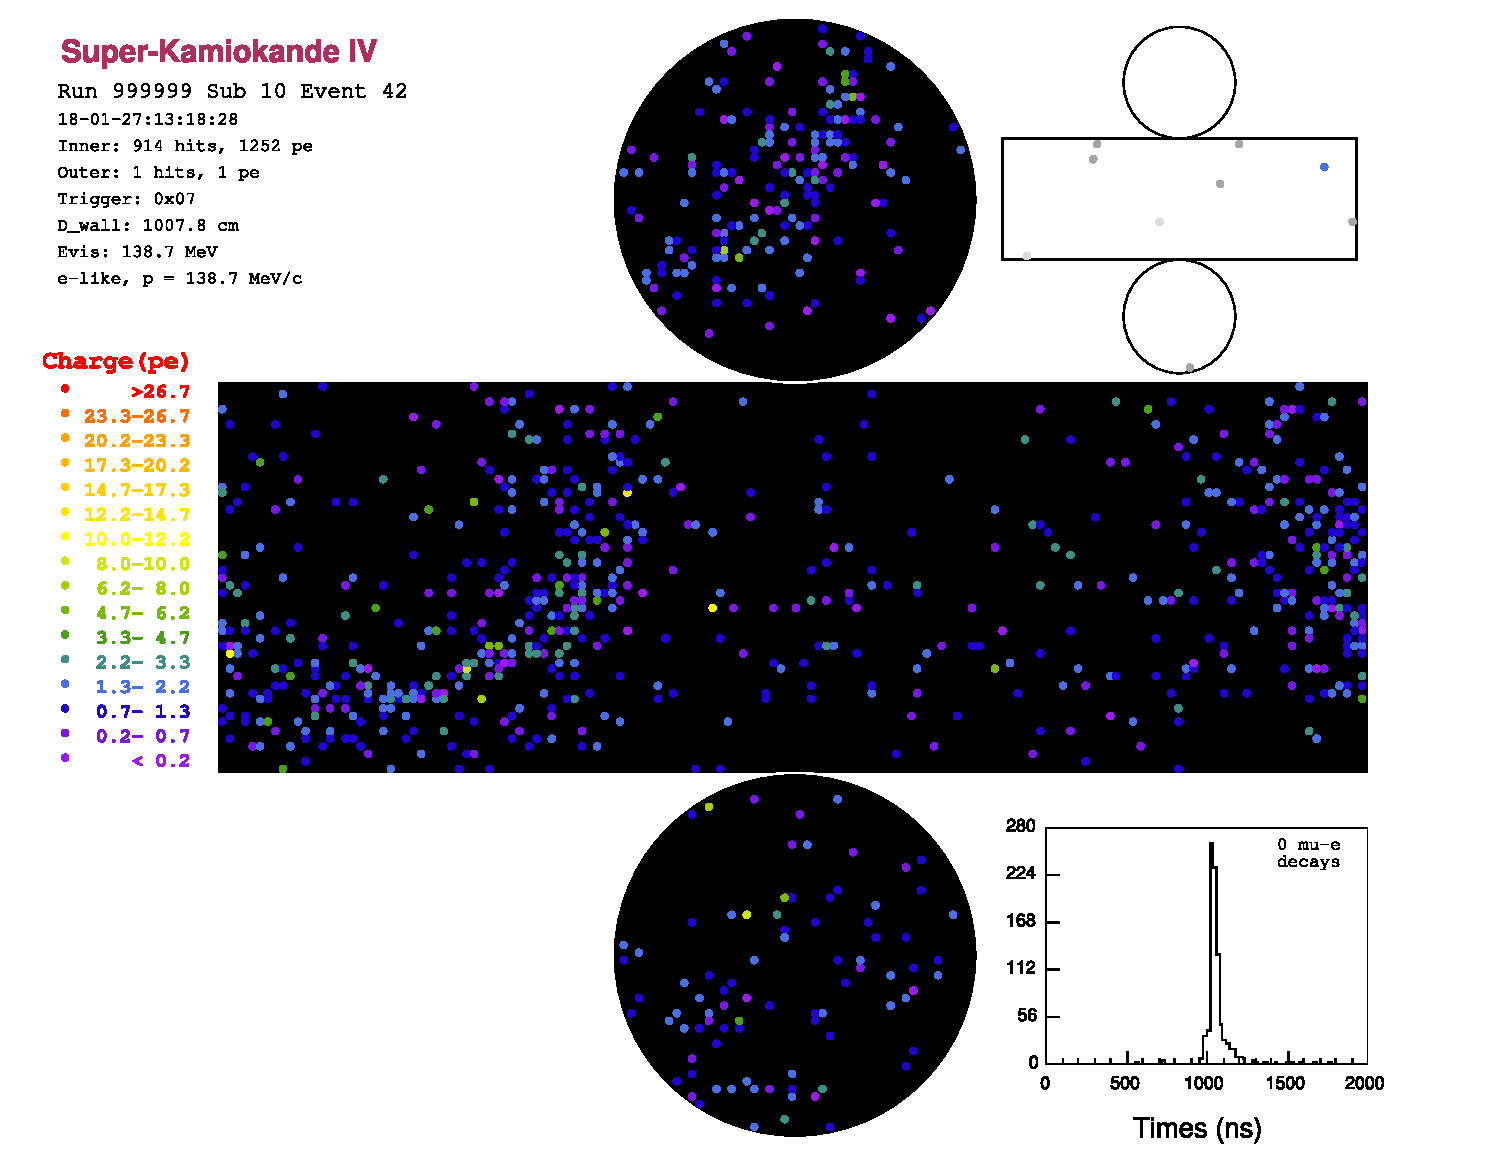
\includegraphics[width=0.45\textwidth]{pics/Electron.pdf}
	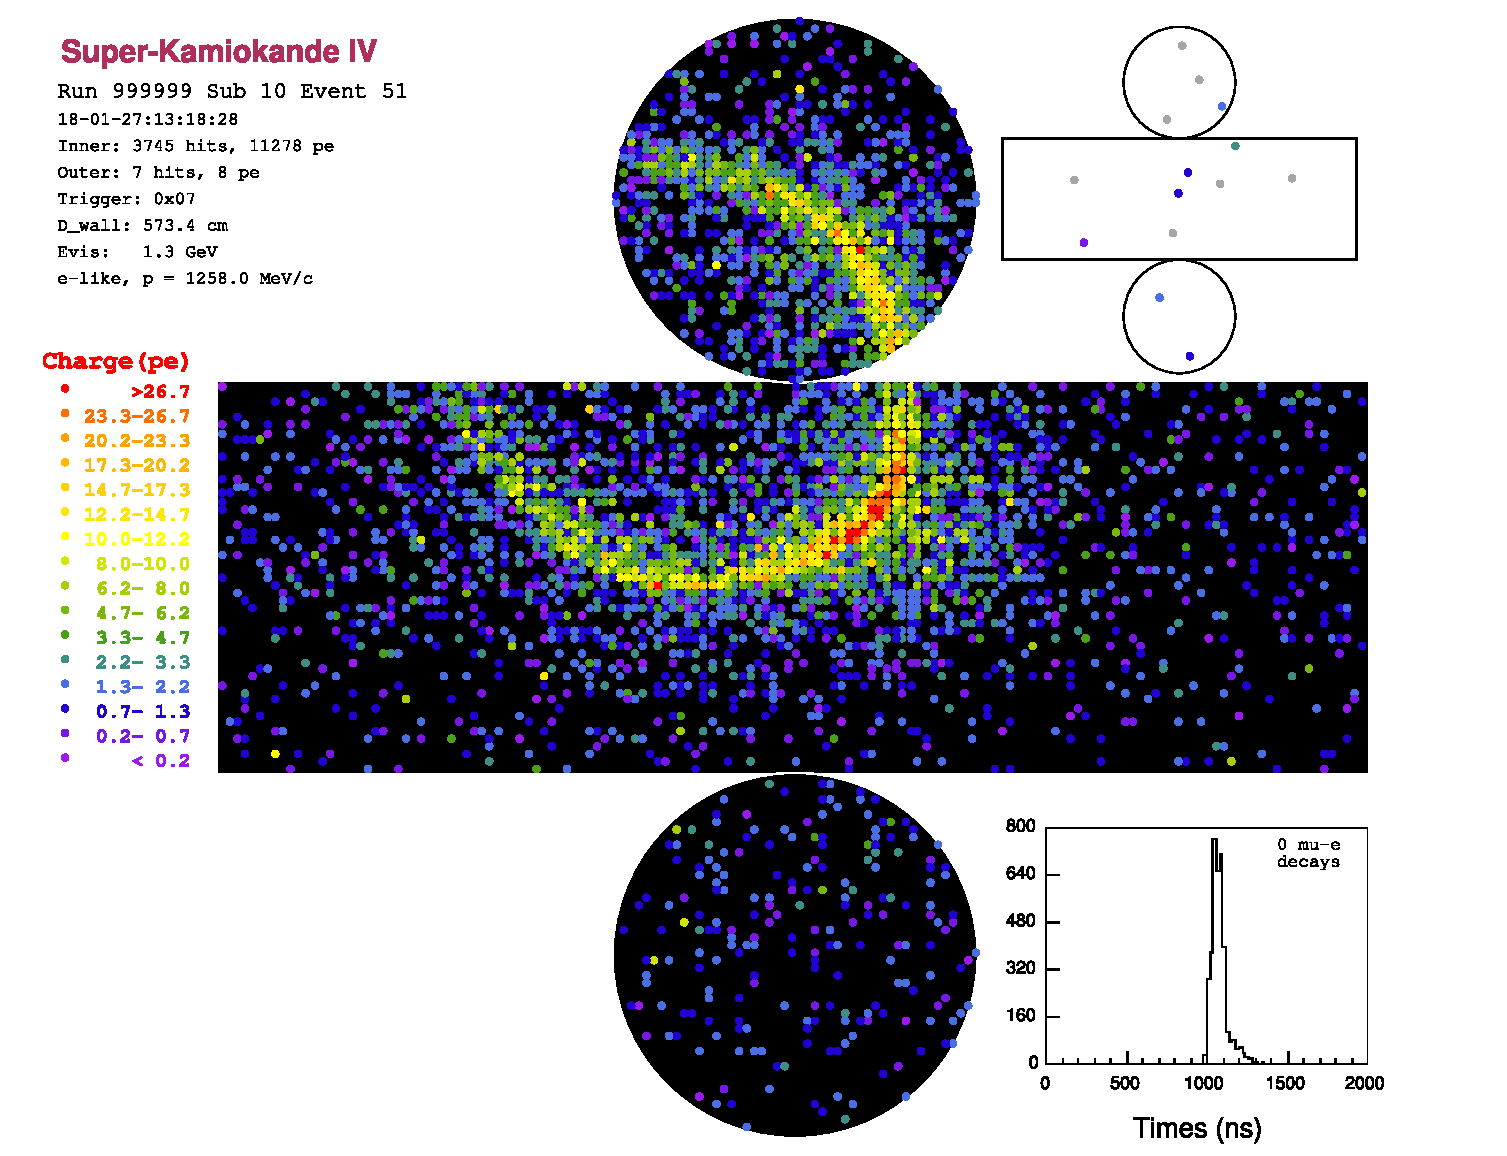
\includegraphics[width=0.45\textwidth]{pics/Muon.pdf}
	\caption{Fully-contained events in the fiducial volume of Super-Kamiokande.}
	\label{fig:sk_events}
\end{figure}

The Super-Kamiokande experiment (SK) is a water Cherenkov detector, %
located in the Kamioka mine, under Mt.\ Ikeno in the Gifu prefecture, Japan.
The rock overburden of $\sim\np{1000}$\,m (\np{2700}\,m.w.e.), shields very efficiently the experiment %
and only cosmic-rays with energies above 1.3\,TeV can reach the detector: %
the muon flux at SK is about \np{6e-8}\,cm\tapi{-2}s\tapi{-1}sr\tapi{-1}, which translates to a rate of 2\,Hz.
The detector consists of a cylindrical stainless steel tank, with a height of 41.4\,m and a diameter of 39.3\,m, %
and it is filled with 50\,kt of ultra pure water.
The water region is separated into two concentric cylindrical regions, %
called the inner detector (ID, 33.8\,m in diameter) and the outer detector (OD), the latter working as passive and active veto.
The two regions are separated a 55\,cm insensitive region containing the support structure for the PMTs and their cables.
The ID is instrumented with \np{11129} 20'' Hamamatsu R3600 PMTs, facing towards the inside of the tank.
Since the 2001 implosion accident, the photocathode of the PMTs are protected by UV--transparent acrylic domes %
and the side with fiber-reinforced plastic.
The photo coverage of the inner surface is around 40\,\%; the remaining surface not occupied by a PMT is %
lined with black sheet to reduce light reflection.
The main goal of the OD is to tag events originating or finishing outside the ID.
It is instrumented with \np{1885} 8'' Hamamatsu R1408 PMTs which are optically coupled to wavelength shifting plates %
to increase light collectionto increases light collection.
Sheets of white tyvek maximise the propagation of photons inside the ID and helps the reconstruction of corner-clipping events.

The refractive index of water in the visible and ultraviolet region is $n \geq 1.33$, %
and so a charged particle can emit Cherenkov radiation if it is travelling %
with speed $\beta \gtrsim 0.75$.
This converts to an energy threshold of \np{0.78}\,MeV for electrons, \np{160.26}\,MeV for muons, %
\np{211.69}\,MeV for pions, and \np{1423.13}\,MeV for protons, which are the particles usually detected in SK.
The Cherenkov photons, thanks to the high-purity water, reach the walls of the tank where they %
are collected by the PMTs, forming ring patterns.
From the time and charge deposited on the PMTs, the event reconstruction algorithm extracts information of the event %
such as vertex, direction, and energy.
%High energy events, for which $\beta \simeq 1$, generates Cherenkov rings with the same conic angle, %
%which is $\theta \simeq 41^\circ$ in water. 
The same algorithm performs particle identification by looking at the topology and the multiplicity of the ring patterns: %
for example, an electron travelling in the water is more likely to be scattered compared to a muon, %
that on the other hand will follow a more straight path, and as a consquence %
the electron-induced ring is less defined and fuzzier than the muon-induced one.
This can be appreciated on the reconstructed events of \reffig{fig:sk_events}.
Pions usually interact hadronically nuclei with oxygen nuclei, and therefore they have shorter %
and the Cherenkov rings are also less defined than a muon ones.
Muon and pion events can be accompanied by secondary rings from the electrons produced in their decays.
Energetic gamma rays can also be detected, as for instance the ones from $\pi^0$ decays, %
through rings of electrons accelerated by Compton scattering.


As part of the strategies to tackle backgrounds, typically only events originating at the centre %
of the ID are considered to be valid.
The materials of the walls of the tank, and particulary the glass of PMTs, contains radioactive material, %
such as isotopes of thorium, uranium and potassium.
These impurities can mimic a signal event in the MeV energy region, crucial for solar neutrino studies.
The selection algorithm simply discards any reconstructed event the vertex of which is less than 200\,cm away from the ID walls.
This criteria defines a fiducial volume (FV), which is around 22.5\,kt in water mass.
The water used to fill the tank may also contain impurities, among which radon, that cause background events.
The water in the tank is continuously filtered at a flow rate of 60\,t/hour by a water purification system (see \refsec{sec:gadolinium}).
An air purification system pumps radon-free air into the SK area inside the mine.
This prevents radon in the air to dissolve in the purified water.
Radon contamination is usually less than 3\,mBq/m\tapi{3}, compared to unpurifies air that can peak %
at about 1200\,Bq/m\tapi{3}.
Thanks to these precautions the current energy threshold for SK is \np{3.5}\,MeV.
The main oscillation analyses of SK consider only events originating inside the FV and fully-contained, %
i.e.\ that do not propagate in the OD, as this is signature is given mostly by neutrino interactions.

\section{Neutrons in Super-Kamiokande}
\label{sec:sk_neutron}

Super-Kamiokande and other large scale water Cherenkov detectors have provided %
many evidences in the experimental understanding of neutrinos, %
be it originated in solar, atmospheric, or accelerator facilities.
Despite the large exposure of the experiment, some studies are still curbed by statistical uncertainty %
and would benefit from simply collecting more data.
Other searches, instead, suffer from irreducible background events, as for example the detection of Relic Supernova Neutrinos (SNR), %
%One of the main motivation to detect neutrons is to be able to detect relic supernova neutrinos, %
also know as Diffuse Supernova Neutrino Background (DSNB), an incoherent background spectrum %
produced from all previous core-collapse supernova explosions in the Universe (see \refsec{sec:nu_sun_sn}).
The observation of SNR would be of great importance for improving our knowledge on the population of core-collapse SN %
and the rate of star formation.
The predictions provide with several limits but although SK has the best world limit, no SRN has been detected yet.
The average energies of these neutrinos are around a few tens of MeV, at which the largest cross-section %
corresponds to inverse beta decay (IBD, see \refsec{sec:ibd}).
%which is two orders of magnitude larger than $\nu_e$ elastic scattering.
This measurement is afflicted at low energies by invisible muon decay%
---muons below Cherenkov threshold that decay into electrons---and at high energies, %
between $14\,\text{MeV} < E_\nu < 30\,\text{MeV}$, by atmospheric neutrinos.
The energy threshold is also limited by muon-induced spallation events and solar neutrinos, that could be successfully %
rejected with neutron tagging.
If we could detect neutrons efficiently, these backgrounds could be reduced significantly and thus, %
making the detection of the DSNB possible for the first time.

Searches of galactic supernova burst could also avail of an improved background suppression.
SK will be exposed to a huge number of neutrino events if a core-collapse supernova occurs inside our galaxy, %
providing not only an early warning system for other observatories (see \refsec{sec:nu_sun_sn}), %
but also information about the neutrino spectrum, time profile, and information about early stages of the core-collapse process, %
such as pre-supernova neutrinos from the silicon burning phase~\cite{Simpson:2019xwo}.
The majority of neutrinos emitted are actually antineutrinos in the energies where IBD cross-section dominates.
Detecting the neutron in the final state can be fundamental in distinguishing whether the incoming particle is %
a neutrino or an antineutrino.

Improved neutron tagging is also helpful to understand atmospheric and accelerator neutrino interactions and final states.
At energies $E_\nu > 1$\,GeV, the number of CCQE interactions decreases and often additional neutrons or pions %
are also released by secondary hadronic interaction.
The capability of separating neutrinos and antineutrinos can still produce anti-neutrino enriched samples
 Finally, the background in proton decay searches can be reduced, since it requires no neutrons to appear in the final state.

%Among these background sources, flasher events\footnote{A flasher event refers to the phenomenon %
%	in which a PMT mis-fires and many repetitive internal discharges are triggered also on nearby PMTs.
%	Flasher events tend to have a broader hit timing distribution than neutrino events.} %

\subsection{Neutron tagging}

Neutrons have a relative long lifetime and since they cannot directly emit Cherenkov radiation, %
these particles can travel quite some distance from they production point.
Neutrons interact with nuclei in various way, depending on their energy and the target nuclues.
The interactions are divided in three typologies: scattering, which can elastic or inelastic, %
absorptions, such as radiative capture or fission, and nucleon transfer reactions.
The kinetic energy of the neutron $T$, sometimes referred to as the \emph{detection temperature}, %
is the main factor in determining the dominant cross-section of these interactions.
For fast neutrons, with $T > 1$\,MeV, elastic scattering is the dominant interaction mode, and %
for some target nuclei the only mode possible.
The cross-section for these energetic neutrons presents some wide resonance peaks which depend %
on the target nuclei.
The elastic scattering cross-sections at energies below 1\,MeV is almost independent of the neutron energy.
This is true for most light isotopes, but some intermediate and heavy elements presents some specific %
behaviour at higher energy.
Neutrons for which $T \simeq \np{0.0025}$\,eV are called \emph{thermal neutrons} because %
a Maxwell-Boltzmann distribution at a temperature 290\,K peaks at that energy; %
such neutrons are therefore in thermal equilibrium with the surrounding medium.
At thermal energies and below the most important interaction is neutron absorption and the cross-section follows the ``$1/v$ law'', %
with $v$ the velocity of the neutron.
In this region, absorption cross-section increases as the velocity, or the detection temperature, of the neutron decreases
\begin{equation}
	\label{eq:abs_xsec}
	\sigma \sim \frac{1}{v} \sim \frac{1}{T}
\end{equation}
Being in thermal equilibrium and having a lower kinetic energy allows the neutron to form %
a compound nucleus with the target, which might undergo fission or radiation emission if it is a non-fissile nuclide.
For energies between a few eV and hundreds of keV, resonances in the capture cross-section occurs and these %
are strongly dependent on the target isotope, but also on the temperature of the material.
The thermal motions of the target relative to the incident neutron broadens the resonance peaks, %
despite the integrated cross-section over the energy remains constant.
This effect is called \emph{Doppler broadening}, and results in a decreased likelihood of capture or fission %
when the target material has a wide energy distribution.

%%https://doi.org/10.1016/j.nds.2018.02.001
%Brown:2018jhj,

Fast neutrons slow down to thermal energies via subsequent elastic collisions, until %
the free neutron is captured by some nuclei.
This process is called \emph{thermalisation}.
Considering a scattering between a neutron and a nucleus, $n + A \to n + A$, %
the final state energy of the neutron depends on the outgoing angle $\hat\theta$ %
in the centre of mass frame
\begin{equation}
	\label{eq:outgoing_E}
	E_\text{f} = E_\text{i}\ \frac{(1+\zeta) + (1 - \zeta) \cos\hat\theta}{2} \ ,
\end{equation}
where $E_\text{i,f}$ are the intial and final energies of the free neutron and $\zeta$ %
is the following kinematic factor
\begin{equation}
	\label{eq:n_alpha}
	\zeta = \frac{(m_n - M_A)^2}{(m_n + M_A)^2} \simeq \frac{(1 - A)^2}{(1 + A)^2}\ .
\end{equation}
Using classic mechanics, in the laboratory frame the scattering angle $\theta$ is given by
\begin{equation}
	\label{eq:lab_angle}
	\cos\theta = \frac{A\,\cos\hat\theta + 1}{\sqrt{1 + 2\,A\,\cos\hat\theta + A^2}}\ ,
\end{equation}
and we can therefore estimate the average scattering angle
\begin{equation}
	\label{eq:average_angle}
	\expval{\cos\theta} = \frac{\displaystyle \int\dd{\Omega} \cos\theta}{\displaystyle \int \dd{\Omega}} = \frac{2}{3 A}\ .
\end{equation}
Heavy targets will deviate on average more the neutron from its path than light targets.
For hydrogen ($A = 1$), the average angle is $\expval{\theta} \simeq 48^\circ$, but %
for heavier elements with large atomic mass, the average angle approximate $\expval{\theta} \to 90^\circ$.
Assuming uniform isotropic scattering, the average outgoing energy for the neutron is
\begin{equation}
	\label{eq:average_outgoing_E}
	\expval{E_\text{f}} = \frac{\displaystyle \int \dd{\Omega} E_\text{f}}{\displaystyle \int\dd{\Omega}} = E_\text{i}\ \frac{1+\zeta}{2}\ .
\end{equation}
This means that if each neutron collision decreses to the same average final state energy, %
after $n$ interactions the neutron energy is
\begin{equation}
	\label{eq:energy_loss}
	E_n = E_0 \qty(\frac{1+\zeta}{2})^n = E_0\,e^{-n \xi}\ .
\end{equation}
The thermalisation process follows an exponential law, and $\xi$ represents the typical %
energy decrease in log-scale, which on average equals to
\begin{equation}
	\label{eq:average_decrease}
	\expval{\xi} = \frac{\displaystyle \int \dd{\Omega} \log\qty(\frac{E_\text{i}}{E_\text{f}})}{\displaystyle \int\dd{\Omega}} %
		     = \frac{\zeta - \zeta \log \zeta -1 }{\zeta - 1} = 1 + \frac{(A-1)^2}{2A} \log \frac{A-1}{A+1}\ .
\end{equation}
With the expression, we can compute the average number of collisions a neutron undergoes when %
propagating in a medium.
Because of the dependency of $\xi$ on $A$, lighter nuclides are more effective than heavier ones.
For example, the number of interactions for a fast neutron to slow down to thermal energies in lead ($A = 208$) %
is about hunderd times the number of interactions that would occur in hydrogen.
In reality, the media in which neutrons propagate are compounds with more than one type of target.
The energy decrease for these materials is an average of the individual components weighted by %
their respective elastic cross-sections
\begin{equation}
	\label{eq:decrease_weighted}
	\xi_\text{tot}(E) = \frac{\sum_k \sigma_k(E) \xi_k(E)}{\sum_k \sigma_k(E)}\ .
\end{equation}
In this simplified scenario we overlooked the impact of resonance capture, which manifests at around the keV energy range.
While fast neutrons with energies above 1\,MeV are being slowed down to thermal energies, %
the mean free path decreases with the neutron's velocity, and the possibility of resonance capture increases.
These captures would affect the relative neutron flux around the energy of the resonance peaks, which %
might be widened by the Doppler broadening effect.

\begin{figure}
	\centering
	\resizebox{\linewidth}{!}{% GNUPLOT: LaTeX picture with Postscript
\begingroup
  \makeatletter
  \providecommand\color[2][]{%
    \GenericError{(gnuplot) \space\space\space\@spaces}{%
      Package color not loaded in conjunction with
      terminal option `colourtext'%
    }{See the gnuplot documentation for explanation.%
    }{Either use 'blacktext' in gnuplot or load the package
      color.sty in LaTeX.}%
    \renewcommand\color[2][]{}%
  }%
  \providecommand\includegraphics[2][]{%
    \GenericError{(gnuplot) \space\space\space\@spaces}{%
      Package graphicx or graphics not loaded%
    }{See the gnuplot documentation for explanation.%
    }{The gnuplot epslatex terminal needs graphicx.sty or graphics.sty.}%
    \renewcommand\includegraphics[2][]{}%
  }%
  \providecommand\rotatebox[2]{#2}%
  \@ifundefined{ifGPcolor}{%
    \newif\ifGPcolor
    \GPcolortrue
  }{}%
  \@ifundefined{ifGPblacktext}{%
    \newif\ifGPblacktext
    \GPblacktexttrue
  }{}%
  % define a \g@addto@macro without @ in the name:
  \let\gplgaddtomacro\g@addto@macro
  % define empty templates for all commands taking text:
  \gdef\gplbacktext{}%
  \gdef\gplfronttext{}%
  \makeatother
  \ifGPblacktext
    % no textcolor at all
    \def\colorrgb#1{}%
    \def\colorgray#1{}%
  \else
    % gray or color?
    \ifGPcolor
      \def\colorrgb#1{\color[rgb]{#1}}%
      \def\colorgray#1{\color[gray]{#1}}%
      \expandafter\def\csname LTw\endcsname{\color{white}}%
      \expandafter\def\csname LTb\endcsname{\color{black}}%
      \expandafter\def\csname LTa\endcsname{\color{black}}%
      \expandafter\def\csname LT0\endcsname{\color[rgb]{1,0,0}}%
      \expandafter\def\csname LT1\endcsname{\color[rgb]{0,1,0}}%
      \expandafter\def\csname LT2\endcsname{\color[rgb]{0,0,1}}%
      \expandafter\def\csname LT3\endcsname{\color[rgb]{1,0,1}}%
      \expandafter\def\csname LT4\endcsname{\color[rgb]{0,1,1}}%
      \expandafter\def\csname LT5\endcsname{\color[rgb]{1,1,0}}%
      \expandafter\def\csname LT6\endcsname{\color[rgb]{0,0,0}}%
      \expandafter\def\csname LT7\endcsname{\color[rgb]{1,0.3,0}}%
      \expandafter\def\csname LT8\endcsname{\color[rgb]{0.5,0.5,0.5}}%
    \else
      % gray
      \def\colorrgb#1{\color{black}}%
      \def\colorgray#1{\color[gray]{#1}}%
      \expandafter\def\csname LTw\endcsname{\color{white}}%
      \expandafter\def\csname LTb\endcsname{\color{black}}%
      \expandafter\def\csname LTa\endcsname{\color{black}}%
      \expandafter\def\csname LT0\endcsname{\color{black}}%
      \expandafter\def\csname LT1\endcsname{\color{black}}%
      \expandafter\def\csname LT2\endcsname{\color{black}}%
      \expandafter\def\csname LT3\endcsname{\color{black}}%
      \expandafter\def\csname LT4\endcsname{\color{black}}%
      \expandafter\def\csname LT5\endcsname{\color{black}}%
      \expandafter\def\csname LT6\endcsname{\color{black}}%
      \expandafter\def\csname LT7\endcsname{\color{black}}%
      \expandafter\def\csname LT8\endcsname{\color{black}}%
    \fi
  \fi
    \setlength{\unitlength}{0.0500bp}%
    \ifx\gptboxheight\undefined%
      \newlength{\gptboxheight}%
      \newlength{\gptboxwidth}%
      \newsavebox{\gptboxtext}%
    \fi%
    \setlength{\fboxrule}{0.5pt}%
    \setlength{\fboxsep}{1pt}%
\begin{picture}(14400.00,5760.00)%
    \gplgaddtomacro\gplbacktext{%
      \csname LTb\endcsname%%
      \put(618,1038){\makebox(0,0)[r]{\strut{}\np{e-4}}}%
      \csname LTb\endcsname%%
      \put(618,1812){\makebox(0,0)[r]{\strut{}\np{e-2}}}%
      \csname LTb\endcsname%%
      \put(618,2586){\makebox(0,0)[r]{\strut{}\np{1}}}%
      \csname LTb\endcsname%%
      \put(618,3359){\makebox(0,0)[r]{\strut{}\np{e2}}}%
      \csname LTb\endcsname%%
      \put(618,4133){\makebox(0,0)[r]{\strut{}\np{e4}}}%
      \csname LTb\endcsname%%
      \put(618,4907){\makebox(0,0)[r]{\strut{}\np{e6}}}%
      \csname LTb\endcsname%%
      \put(1100,465){\makebox(0,0){\strut{}\np{e-4}}}%
      \csname LTb\endcsname%%
      \put(1860,465){\makebox(0,0){\strut{}\np{e-2}}}%
      \csname LTb\endcsname%%
      \put(2620,465){\makebox(0,0){\strut{}1}}%
      \csname LTb\endcsname%%
      \put(3379,465){\makebox(0,0){\strut{}\np{e2}}}%
      \csname LTb\endcsname%%
      \put(4139,465){\makebox(0,0){\strut{}\np{e4}}}%
      \csname LTb\endcsname%%
      \put(4899,465){\makebox(0,0){\strut{}\np{e6}}}%
    }%
    \gplgaddtomacro\gplfronttext{%
      \csname LTb\endcsname%%
      \put(126,2972){\rotatebox{-270}{\makebox(0,0){\strut{}Cross-section (b)}}}%
      \csname LTb\endcsname%%
      \put(2999,186){\makebox(0,0){\strut{}Energy (eV)}}%
      \csname LTb\endcsname%%
      \put(2999,5573){\makebox(0,0){\strut{}Hydrogen \tapi{1}H}}%
      \csname LTb\endcsname%%
      \put(4746,5127){\makebox(0,0)[r]{\strut{}Total}}%
      \csname LTb\endcsname%%
      \put(4746,4941){\makebox(0,0)[r]{\strut{}Elastic}}%
      \csname LTb\endcsname%%
      \put(4746,4755){\makebox(0,0)[r]{\strut{}Capture}}%
      \csname LTb\endcsname%%
      \put(618,1038){\makebox(0,0)[r]{\strut{}\np{e-4}}}%
      \csname LTb\endcsname%%
      \put(618,1812){\makebox(0,0)[r]{\strut{}\np{e-2}}}%
      \csname LTb\endcsname%%
      \put(618,2586){\makebox(0,0)[r]{\strut{}1}}%
      \csname LTb\endcsname%%
      \put(618,3359){\makebox(0,0)[r]{\strut{}\np{e2}}}%
      \csname LTb\endcsname%%
      \put(618,4133){\makebox(0,0)[r]{\strut{}\np{e4}}}%
      \csname LTb\endcsname%%
      \put(618,4907){\makebox(0,0)[r]{\strut{}\np{e6}}}%
      \csname LTb\endcsname%%
      \put(1100,465){\makebox(0,0){\strut{}\np{e-4}}}%
      \csname LTb\endcsname%%
      \put(1860,465){\makebox(0,0){\strut{}\np{e-2}}}%
      \csname LTb\endcsname%%
      \put(2620,465){\makebox(0,0){\strut{}1}}%
      \csname LTb\endcsname%%
      \put(3379,465){\makebox(0,0){\strut{}\np{e2}}}%
      \csname LTb\endcsname%%
      \put(4139,465){\makebox(0,0){\strut{}\np{e4}}}%
      \csname LTb\endcsname%%
      \put(4899,465){\makebox(0,0){\strut{}\np{e6}}}%
    }%
    \gplgaddtomacro\gplbacktext{%
      \csname LTb\endcsname%%
      \put(5178,1038){\makebox(0,0)[r]{\strut{}}}%
      \csname LTb\endcsname%%
      \put(5178,1812){\makebox(0,0)[r]{\strut{}}}%
      \csname LTb\endcsname%%
      \put(5178,2586){\makebox(0,0)[r]{\strut{}}}%
      \csname LTb\endcsname%%
      \put(5178,3359){\makebox(0,0)[r]{\strut{}}}%
      \csname LTb\endcsname%%
      \put(5178,4133){\makebox(0,0)[r]{\strut{}}}%
      \csname LTb\endcsname%%
      \put(5178,4907){\makebox(0,0)[r]{\strut{}}}%
      \csname LTb\endcsname%%
      \put(5280,465){\makebox(0,0){\strut{}\np{e-5}}}%
      \csname LTb\endcsname%%
      \put(6036,465){\makebox(0,0){\strut{}\np{e-4}}}%
      \csname LTb\endcsname%%
      \put(6791,465){\makebox(0,0){\strut{}\np{e-3}}}%
      \csname LTb\endcsname%%
      \put(7547,465){\makebox(0,0){\strut{}\np{e-2}}}%
      \csname LTb\endcsname%%
      \put(8303,465){\makebox(0,0){\strut{}\np{0.1}}}%
      \csname LTb\endcsname%%
      \put(9058,465){\makebox(0,0){\strut{}\np{1}}}%
      \csname LTb\endcsname%%
      \put(9814,465){\makebox(0,0){\strut{}10}}%
      \csname LTb\endcsname%%
      \put(10570,465){\makebox(0,0){\strut{}\np{e2}}}%
      \csname LTb\endcsname%%
      \put(11325,465){\makebox(0,0){\strut{}\np{e3}}}%
      \csname LTb\endcsname%%
      \put(12081,465){\makebox(0,0){\strut{}\np{e4}}}%
      \csname LTb\endcsname%%
      \put(12837,465){\makebox(0,0){\strut{}\np{e5}}}%
      \csname LTb\endcsname%%
      \put(13592,465){\makebox(0,0){\strut{}\np{e6}}}%
      \csname LTb\endcsname%%
      \put(14348,465){\makebox(0,0){\strut{}\np{e7}}}%
    }%
    \gplgaddtomacro\gplfronttext{%
      \csname LTb\endcsname%%
      \put(5178,2972){\rotatebox{-270}{\makebox(0,0){\strut{}}}}%
      \csname LTb\endcsname%%
      \put(9814,186){\makebox(0,0){\strut{}Energy (eV)}}%
      \csname LTb\endcsname%%
      \put(9814,5573){\makebox(0,0){\strut{}Gadolinium \tapi{157}Gd}}%
      \csname LTb\endcsname%%
      \put(13815,5127){\makebox(0,0)[r]{\strut{}Total}}%
      \csname LTb\endcsname%%
      \put(13815,4941){\makebox(0,0)[r]{\strut{}Elastic}}%
      \csname LTb\endcsname%%
      \put(13815,4755){\makebox(0,0)[r]{\strut{}Capture}}%
      \csname LTb\endcsname%%
      \put(5178,1038){\makebox(0,0)[r]{\strut{}}}%
      \csname LTb\endcsname%%
      \put(5178,1812){\makebox(0,0)[r]{\strut{}}}%
      \csname LTb\endcsname%%
      \put(5178,2586){\makebox(0,0)[r]{\strut{}}}%
      \csname LTb\endcsname%%
      \put(5178,3359){\makebox(0,0)[r]{\strut{}}}%
      \csname LTb\endcsname%%
      \put(5178,4133){\makebox(0,0)[r]{\strut{}}}%
      \csname LTb\endcsname%%
      \put(5178,4907){\makebox(0,0)[r]{\strut{}}}%
      \csname LTb\endcsname%%
      \put(5280,465){\makebox(0,0){\strut{}\np{e-5}}}%
      \csname LTb\endcsname%%
      \put(6036,465){\makebox(0,0){\strut{}\np{e-4}}}%
      \csname LTb\endcsname%%
      \put(6791,465){\makebox(0,0){\strut{}\np{e-3}}}%
      \csname LTb\endcsname%%
      \put(7547,465){\makebox(0,0){\strut{}\np{e-2}}}%
      \csname LTb\endcsname%%
      \put(8303,465){\makebox(0,0){\strut{}\np{0.1}}}%
      \csname LTb\endcsname%%
      \put(9058,465){\makebox(0,0){\strut{}\np{1}}}%
      \csname LTb\endcsname%%
      \put(9814,465){\makebox(0,0){\strut{}\np{10}}}%
      \csname LTb\endcsname%%
      \put(10570,465){\makebox(0,0){\strut{}\np{e2}}}%
      \csname LTb\endcsname%%
      \put(11325,465){\makebox(0,0){\strut{}\np{e3}}}%
      \csname LTb\endcsname%%
      \put(12081,465){\makebox(0,0){\strut{}\np{e4}}}%
      \csname LTb\endcsname%%
      \put(12837,465){\makebox(0,0){\strut{}\np{e5}}}%
      \csname LTb\endcsname%%
      \put(13592,465){\makebox(0,0){\strut{}\np{e6}}}%
      \csname LTb\endcsname%%
      \put(14348,465){\makebox(0,0){\strut{}\np{e7}}}%
    }%
    \iffalse
    \gplgaddtomacro\gplbacktext{%
      \csname LTb\endcsname%%
      \put(8717,864){\makebox(0,0)[l]{\strut{}0.1}}%
      \csname LTb\endcsname%%
      \put(8717,1382){\makebox(0,0)[l]{\strut{}1}}%
      \csname LTb\endcsname%%
      \put(8717,1900){\makebox(0,0)[l]{\strut{}10}}%
      \csname LTb\endcsname%%
      \put(8717,2419){\makebox(0,0)[l]{\strut{}\np{e2}}}%
      \csname LTb\endcsname%%
      \put(8717,2937){\makebox(0,0)[l]{\strut{}\np{e3}}}%
      \csname LTb\endcsname%%
      \put(8717,3455){\makebox(0,0)[l]{\strut{}\np{e4}}}%
      \csname LTb\endcsname%%
      \put(5989,3641){\makebox(0,0){\strut{}20}}%
      \csname LTb\endcsname%%
      \put(6737,3641){\makebox(0,0){\strut{}50}}%
      \csname LTb\endcsname%%
      \put(7868,3641){\makebox(0,0){\strut{}200}}%
      \csname LTb\endcsname%%
      \put(8615,3641){\makebox(0,0){\strut{}500}}%
      \csname LTb\endcsname%%
      \put(5424,3641){\makebox(0,0){\strut{}10}}%
      \csname LTb\endcsname%%
      \put(7302,3641){\makebox(0,0){\strut{}100}}%
    }%
    \fi
    \gplgaddtomacro\gplfronttext{%
      \csname LTb\endcsname%%
      \put(5433,2159){\rotatebox{-270}{\makebox(0,0){\strut{}}}}%
      \csname LTb\endcsname%%
      \put(7019,808){\makebox(0,0){\strut{}}}%
      \csname LTb\endcsname%%
      \put(7019,3548){\makebox(0,0){\strut{}}}%
      \csname LTb\endcsname%%
      \put(8717,864){\makebox(0,0)[l]{\strut{}0.1}}%
      \csname LTb\endcsname%%
      \put(8717,1382){\makebox(0,0)[l]{\strut{}1}}%
      \csname LTb\endcsname%%
      \put(8717,1900){\makebox(0,0)[l]{\strut{}10}}%
      \csname LTb\endcsname%%
      \put(8717,2419){\makebox(0,0)[l]{\strut{}\np{e2}}}%
      \csname LTb\endcsname%%
      \put(8717,2937){\makebox(0,0)[l]{\strut{}\np{e3}}}%
      \csname LTb\endcsname%%
      \put(8717,3455){\makebox(0,0)[l]{\strut{}\np{e4}}}%
      \csname LTb\endcsname%%
      \put(5989,3641){\makebox(0,0){\strut{}20}}%
      \csname LTb\endcsname%%
      \put(6737,3641){\makebox(0,0){\strut{}50}}%
      \csname LTb\endcsname%%
      \put(7868,3641){\makebox(0,0){\strut{}200}}%
      \csname LTb\endcsname%%
      \put(8615,3641){\makebox(0,0){\strut{}500}}%
      \csname LTb\endcsname%%
      \put(5424,3641){\makebox(0,0){\strut{}10}}%
      \csname LTb\endcsname%%
      \put(7302,3641){\makebox(0,0){\strut{}100}}%
    }%
    \gplbacktext
    \put(0,0){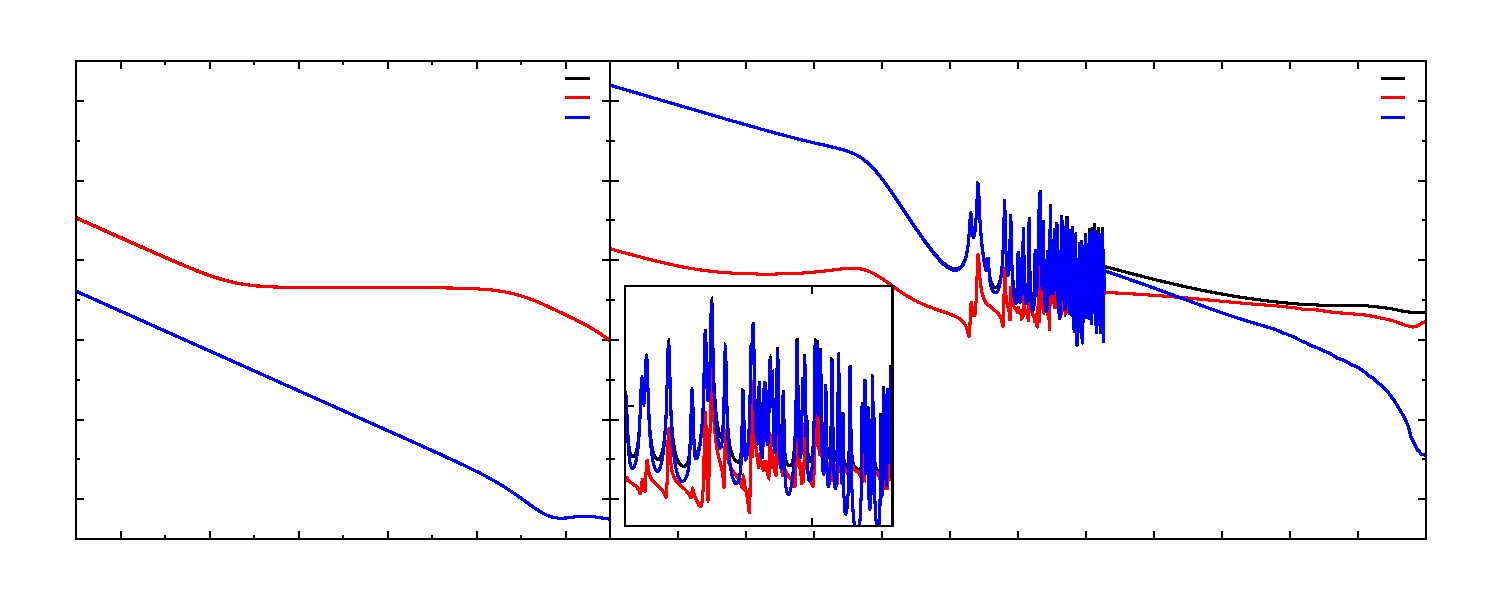
\includegraphics{pics/neutron_xsec}}%
    \gplfronttext
  \end{picture}%
\endgroup
}
	\caption{Neutron cross-sections on hydrogen (left) and gadolinium (right) as a function of energy. %
	       The dominant component for \tapi{1}H is elastic scattering, despite neutron capture %
	       reaches relative high cross-section values for sub-thermal neutrons ($T < 2.5$\,meV).
	       Fast neutrons interact on \tapi{155}Gd via elastic scattering, but for lower energies %
	       the main contribution comes from neutron capture cross-section.
	       The $1/v$ dependency can be appreciated in both cases.
	       The inset shows a detail of the resonance region of the cross-section, %
	       between 10\,eV and 100\,eV.}
	\label{fig:n_xsec}
\end{figure}


From the considerations above, we can deduce that water is a good moderator for thermalising fast neutrons.
The energy decrease for water is $\xi_{\text{H}_2\text{O}} \simeq 0.93$, %
when the kinetic energy of the neutron is in the range $2.5\,\text{meV} \lesssim T \lesssim 0.1\,\text{MeV}$.
Neutrons that reach sub-thermal energies enter the $1/v$ regions in which the capture probabilities increases as $T^{-1}$.
Hydrogen presents a relative high cross-section for neutron capture, as it can be seen from~\reffig{fig:n_xsec}: %
the cross-section for a thermal neutron on hydrogen is measured to be $\np{332.6}$~\,mb~\cite{ZERKIN201831}. %
The cross-section of capture on the oxygen nucleus \tapi{16}O is around $0.19$~\,mb, four orders of magnitude smaller %
than the capture on hydrogen.
The hydrogen capture is followed by the emission of a $\np{2.2}$\,MeV gammas from the %
deexctiation of the newly-formed deuterium.
The characteristic time for Maxwellian nuetrons with energy below 10\,MeV to thermalise and being captured %
by hydrogen in water has been measured to be $(\np{204.8}\pm\np{0.4})$\,\textmu s~\cite{Cokinos:1977zz}.
The typical time and energy of this event require special triggers and dedicated analysis %
to correctly identify the neutron capture on hydrogen in SK.
Since the SK-IV phase, after any primary events above a fixed, higher threshold is detected, 
a time window of 535\,\textmu s is saved with no threshold requirement, so that approximately the 92\,\% %
of neutron capture signals are collected.
The 2.2\,MeV $\gamma$, on average, produces 7$\sim$8 PMT hits, which are difficult to reconstruct accurately.
The PMT hits are expected to happen in a narrow timing distribution and to be anisotropic.
A 10\,ns sliding window is used to look for $\gamma$ candidates with more than 7 hits and less than 50 %
to avoid high energy backgrounds.
With these simple selection criteria, an efficiency of 33.2\,\% is obtained from a simulation of neutron capture events, %
with an expected 4.5 background events per neutrino event.
The background rejection is improved by feeding the simulated data of the selected candidates %
to a neural network, wich retains an overall efficiency of 20.5\,\% with \np{0.018} backgrounds per signal event~\cite{Irvine:2014hja}.
The efficiency is found to be highly dependent on the distance travelled by the released neutron, %
due to the fact that knowning the location of the capture significantly reduce the background.

%follows an exponential and the time constant is largely studied amongst all the thermalisation in water.
%It was found that neutron thermalisation in water has a time constant of 5$\mu$s [fujino, sumita, shiba].
%Neutrons can be captured by either the hydrogen or the oxygen.
%Free neutron will capture on a hydrogen nucleus, releasing a 2.2 MeV gamma.
%In SK, for instance, this gamma results in about seven photo-electrons, and thus only detectable with $\simeq$20\,\% %
%efficiency.

\subsection{Neutron calibration}

%https://arxiv.org/pdf/0811.0735.pdf
%https://www.sno.phy.queensu.ca/sno/papers/labranche_phd.pdf
%https://www.sno.phy.queensu.ca/sno/papers/lyon_phd.pdf

Neutron tagging efficiency in SK has been measured with an americium-beryllium (Am-Be) source~\cite{Watanabe:2008ru}.
In an Am-Be source, \tapi{214}Am decays 100\,\% of the times into \tapi{237}Np via $\alpha$ emission, %
with a half-life of 432.6\,y.
The $\alpha$ particle is captured by the \tapi{9}Be nuclei to become \tapi{12}C\tapi{*} with the emission of a neutron.
The carbon deexcites to the ground state with sometimes the emission of a 4.43\,MeV photon.
This gamma is used to trigger the neutron emission.
The Am-Be source is placed at the centre of a 5\,cm cube of bismuth germanite (BGO) crystal scintillator and %
the device is lowered inside the water Cherenkov tank.
The gamma ray from the beryllium neutron capture is promptly absorbed by the BGO crystal, %
with the release of scintillation light that triggers the detectors. 
Around a thousands of photoelectrons are typically observed by the PMTs from the BGO emission; %
this intense signal triggers the search for neutron captures on hydrogen.
%Forced triggers were imposed during the SK-III phase to extend the acquisition time window.
The candidates are selected by an analysis similary to the simulation study.
Neutrons from beryllium have energies below 10\,MeV, as seen in \reffig{fig:spectra}, %
less than the typical neutron energy resulting from an atmospheric neutrino interactions.
For this reason, in the calibration analysis the neutron capture vertex is assumed to be roughly at the same location %
of the Am-Be source.
The efficiency measured in \refref{Watanabe:2008ru} range from 13.1\,\% to 24.5\,\%, %
the exact value of which is position dependent.
The values agree with the simulation analysis.

\begin{figure}
	\begin{minipage}[t]{0.48\textwidth}
		\centering
		\resizebox{\textwidth}{!}{% GNUPLOT: LaTeX picture with Postscript
\begingroup
  \makeatletter
  \providecommand\color[2][]{%
    \GenericError{(gnuplot) \space\space\space\@spaces}{%
      Package color not loaded in conjunction with
      terminal option `colourtext'%
    }{See the gnuplot documentation for explanation.%
    }{Either use 'blacktext' in gnuplot or load the package
      color.sty in LaTeX.}%
    \renewcommand\color[2][]{}%
  }%
  \providecommand\includegraphics[2][]{%
    \GenericError{(gnuplot) \space\space\space\@spaces}{%
      Package graphicx or graphics not loaded%
    }{See the gnuplot documentation for explanation.%
    }{The gnuplot epslatex terminal needs graphicx.sty or graphics.sty.}%
    \renewcommand\includegraphics[2][]{}%
  }%
  \providecommand\rotatebox[2]{#2}%
  \@ifundefined{ifGPcolor}{%
    \newif\ifGPcolor
    \GPcolortrue
  }{}%
  \@ifundefined{ifGPblacktext}{%
    \newif\ifGPblacktext
    \GPblacktexttrue
  }{}%
  % define a \g@addto@macro without @ in the name:
  \let\gplgaddtomacro\g@addto@macro
  % define empty templates for all commands taking text:
  \gdef\gplbacktext{}%
  \gdef\gplfronttext{}%
  \makeatother
  \ifGPblacktext
    % no textcolor at all
    \def\colorrgb#1{}%
    \def\colorgray#1{}%
  \else
    % gray or color?
    \ifGPcolor
      \def\colorrgb#1{\color[rgb]{#1}}%
      \def\colorgray#1{\color[gray]{#1}}%
      \expandafter\def\csname LTw\endcsname{\color{white}}%
      \expandafter\def\csname LTb\endcsname{\color{black}}%
      \expandafter\def\csname LTa\endcsname{\color{black}}%
      \expandafter\def\csname LT0\endcsname{\color[rgb]{1,0,0}}%
      \expandafter\def\csname LT1\endcsname{\color[rgb]{0,1,0}}%
      \expandafter\def\csname LT2\endcsname{\color[rgb]{0,0,1}}%
      \expandafter\def\csname LT3\endcsname{\color[rgb]{1,0,1}}%
      \expandafter\def\csname LT4\endcsname{\color[rgb]{0,1,1}}%
      \expandafter\def\csname LT5\endcsname{\color[rgb]{1,1,0}}%
      \expandafter\def\csname LT6\endcsname{\color[rgb]{0,0,0}}%
      \expandafter\def\csname LT7\endcsname{\color[rgb]{1,0.3,0}}%
      \expandafter\def\csname LT8\endcsname{\color[rgb]{0.5,0.5,0.5}}%
    \else
      % gray
      \def\colorrgb#1{\color{black}}%
      \def\colorgray#1{\color[gray]{#1}}%
      \expandafter\def\csname LTw\endcsname{\color{white}}%
      \expandafter\def\csname LTb\endcsname{\color{black}}%
      \expandafter\def\csname LTa\endcsname{\color{black}}%
      \expandafter\def\csname LT0\endcsname{\color{black}}%
      \expandafter\def\csname LT1\endcsname{\color{black}}%
      \expandafter\def\csname LT2\endcsname{\color{black}}%
      \expandafter\def\csname LT3\endcsname{\color{black}}%
      \expandafter\def\csname LT4\endcsname{\color{black}}%
      \expandafter\def\csname LT5\endcsname{\color{black}}%
      \expandafter\def\csname LT6\endcsname{\color{black}}%
      \expandafter\def\csname LT7\endcsname{\color{black}}%
      \expandafter\def\csname LT8\endcsname{\color{black}}%
    \fi
  \fi
    \setlength{\unitlength}{0.0500bp}%
    \ifx\gptboxheight\undefined%
      \newlength{\gptboxheight}%
      \newlength{\gptboxwidth}%
      \newsavebox{\gptboxtext}%
    \fi%
    \setlength{\fboxrule}{0.5pt}%
    \setlength{\fboxsep}{1pt}%
\begin{picture}(7200.00,5040.00)%
    \gplgaddtomacro\gplbacktext{%
      \csname LTb\endcsname%%
      \put(747,595){\makebox(0,0)[r]{\strut{}$10^{-4}$}}%
      \csname LTb\endcsname%%
      \put(747,2014){\makebox(0,0)[r]{\strut{}$10^{-3}$}}%
      \csname LTb\endcsname%%
      \put(747,3434){\makebox(0,0)[r]{\strut{}$10^{-2}$}}%
      \csname LTb\endcsname%%
      \put(747,4853){\makebox(0,0)[r]{\strut{}$10^{-1}$}}%
      \csname LTb\endcsname%%
      \put(849,409){\makebox(0,0){\strut{}$0$}}%
      \csname LTb\endcsname%%
      \put(1856,409){\makebox(0,0){\strut{}$2$}}%
      \csname LTb\endcsname%%
      \put(2864,409){\makebox(0,0){\strut{}$4$}}%
      \csname LTb\endcsname%%
      \put(3871,409){\makebox(0,0){\strut{}$6$}}%
      \csname LTb\endcsname%%
      \put(4878,409){\makebox(0,0){\strut{}$8$}}%
      \csname LTb\endcsname%%
      \put(5886,409){\makebox(0,0){\strut{}$10$}}%
      \csname LTb\endcsname%%
      \put(6893,409){\makebox(0,0){\strut{}$12$}}%
    }%
    \gplgaddtomacro\gplfronttext{%
      \csname LTb\endcsname%%
      \put(153,2724){\rotatebox{-270}{\makebox(0,0){\strut{}Distribution}}}%
      \csname LTb\endcsname%%
      \put(3871,130){\makebox(0,0){\strut{}Energy (MeV)}}%
      \csname LTb\endcsname%%
      \put(6411,4081){\makebox(0,0)[r]{\strut{}\tapi{252}Cf $-\ \gamma$}}%
      \csname LTb\endcsname%%
      \put(6411,4360){\makebox(0,0)[r]{\strut{}\tapi{252}Cf $-\ n$}}%
      \csname LTb\endcsname%%
      \put(6411,4639){\makebox(0,0)[r]{\strut{}AmBe $-\ n$}}%
    }%
    \gplbacktext
    \put(0,0){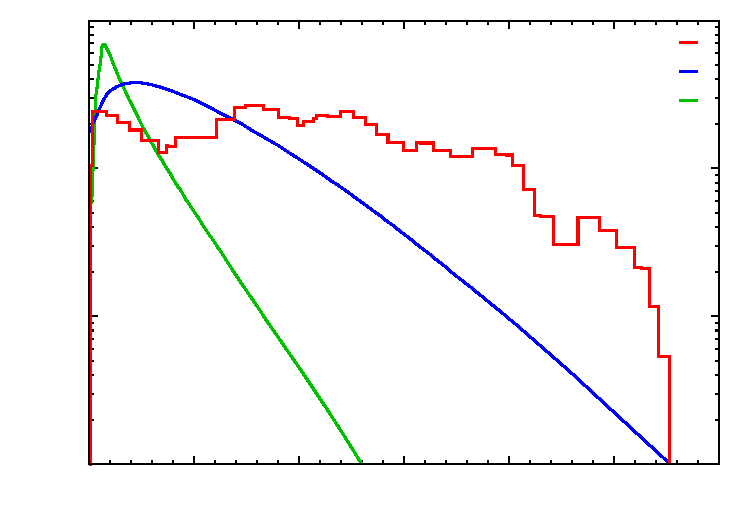
\includegraphics{pics/source_spectrum}}%
    \gplfronttext
  \end{picture}%
\endgroup
}
		\caption{Normalised energy distribution of neutrons emitted by an AmBe source~\cite{PMID:4744412} %
			and neutrons and photons from the spontaneous fission of a %
			\tapi{252}Cf source~\cite{PhysRev.104.699, PhysRev.108.411}.}
		\label{fig:spectra}
	\end{minipage}
	\hfill
	\begin{minipage}[t]{0.48\textwidth}
		\centering
		\resizebox{\textwidth}{!}{% GNUPLOT: LaTeX picture with Postscript
\begingroup
  \makeatletter
  \providecommand\color[2][]{%
    \GenericError{(gnuplot) \space\space\space\@spaces}{%
      Package color not loaded in conjunction with
      terminal option `colourtext'%
    }{See the gnuplot documentation for explanation.%
    }{Either use 'blacktext' in gnuplot or load the package
      color.sty in LaTeX.}%
    \renewcommand\color[2][]{}%
  }%
  \providecommand\includegraphics[2][]{%
    \GenericError{(gnuplot) \space\space\space\@spaces}{%
      Package graphicx or graphics not loaded%
    }{See the gnuplot documentation for explanation.%
    }{The gnuplot epslatex terminal needs graphicx.sty or graphics.sty.}%
    \renewcommand\includegraphics[2][]{}%
  }%
  \providecommand\rotatebox[2]{#2}%
  \@ifundefined{ifGPcolor}{%
    \newif\ifGPcolor
    \GPcolortrue
  }{}%
  \@ifundefined{ifGPblacktext}{%
    \newif\ifGPblacktext
    \GPblacktexttrue
  }{}%
  % define a \g@addto@macro without @ in the name:
  \let\gplgaddtomacro\g@addto@macro
  % define empty templates for all commands taking text:
  \gdef\gplbacktext{}%
  \gdef\gplfronttext{}%
  \makeatother
  \ifGPblacktext
    % no textcolor at all
    \def\colorrgb#1{}%
    \def\colorgray#1{}%
  \else
    % gray or color?
    \ifGPcolor
      \def\colorrgb#1{\color[rgb]{#1}}%
      \def\colorgray#1{\color[gray]{#1}}%
      \expandafter\def\csname LTw\endcsname{\color{white}}%
      \expandafter\def\csname LTb\endcsname{\color{black}}%
      \expandafter\def\csname LTa\endcsname{\color{black}}%
      \expandafter\def\csname LT0\endcsname{\color[rgb]{1,0,0}}%
      \expandafter\def\csname LT1\endcsname{\color[rgb]{0,1,0}}%
      \expandafter\def\csname LT2\endcsname{\color[rgb]{0,0,1}}%
      \expandafter\def\csname LT3\endcsname{\color[rgb]{1,0,1}}%
      \expandafter\def\csname LT4\endcsname{\color[rgb]{0,1,1}}%
      \expandafter\def\csname LT5\endcsname{\color[rgb]{1,1,0}}%
      \expandafter\def\csname LT6\endcsname{\color[rgb]{0,0,0}}%
      \expandafter\def\csname LT7\endcsname{\color[rgb]{1,0.3,0}}%
      \expandafter\def\csname LT8\endcsname{\color[rgb]{0.5,0.5,0.5}}%
    \else
      % gray
      \def\colorrgb#1{\color{black}}%
      \def\colorgray#1{\color[gray]{#1}}%
      \expandafter\def\csname LTw\endcsname{\color{white}}%
      \expandafter\def\csname LTb\endcsname{\color{black}}%
      \expandafter\def\csname LTa\endcsname{\color{black}}%
      \expandafter\def\csname LT0\endcsname{\color{black}}%
      \expandafter\def\csname LT1\endcsname{\color{black}}%
      \expandafter\def\csname LT2\endcsname{\color{black}}%
      \expandafter\def\csname LT3\endcsname{\color{black}}%
      \expandafter\def\csname LT4\endcsname{\color{black}}%
      \expandafter\def\csname LT5\endcsname{\color{black}}%
      \expandafter\def\csname LT6\endcsname{\color{black}}%
      \expandafter\def\csname LT7\endcsname{\color{black}}%
      \expandafter\def\csname LT8\endcsname{\color{black}}%
    \fi
  \fi
    \setlength{\unitlength}{0.0500bp}%
    \ifx\gptboxheight\undefined%
      \newlength{\gptboxheight}%
      \newlength{\gptboxwidth}%
      \newsavebox{\gptboxtext}%
    \fi%
    \setlength{\fboxrule}{0.5pt}%
    \setlength{\fboxsep}{1pt}%
\begin{picture}(7200.00,5040.00)%
    \gplgaddtomacro\gplbacktext{%
      \csname LTb\endcsname%%
      \put(946,2142){\makebox(0,0)[r]{\strut{}$0.05$}}%
      \put(946,4200){\makebox(0,0)[r]{\strut{}$0.5$}}%
      \put(946,704){\makebox(0,0)[r]{\strut{}$0.01$}}%
      \put(946,2762){\makebox(0,0)[r]{\strut{}$0.1$}}%
      \put(946,4819){\makebox(0,0)[r]{\strut{}$1$}}%
      \put(1460,484){\makebox(0,0){\strut{}$300$}}%
      \put(2223,484){\makebox(0,0){\strut{}$350$}}%
      \put(2986,484){\makebox(0,0){\strut{}$400$}}%
      \put(3750,484){\makebox(0,0){\strut{}$450$}}%
      \put(4513,484){\makebox(0,0){\strut{}$500$}}%
      \put(5276,484){\makebox(0,0){\strut{}$550$}}%
      \put(6040,484){\makebox(0,0){\strut{}$600$}}%
      \put(6803,484){\makebox(0,0){\strut{}$650$}}%
    }%
    \gplgaddtomacro\gplfronttext{%
      \csname LTb\endcsname%%
      \put(198,2761){\rotatebox{-270}{\makebox(0,0){\strut{}Efficiency}}}%
      \put(3940,154){\makebox(0,0){\strut{}Wavelength (nm)}}%
      \csname LTb\endcsname%%
      \put(6212,4624){\makebox(0,0)[r]{\strut{}PMT}}%
      \csname LTb\endcsname%%
      \put(6212,4360){\makebox(0,0)[r]{\strut{}Scintillator}}%
      \csname LTb\endcsname%%
      \put(6212,4096){\makebox(0,0)[r]{\strut{}Correlation}}%
      \csname LTb\endcsname%%
      \put(6212,3832){\makebox(0,0)[r]{\strut{}MC}}%
    }%
    \gplbacktext
    \put(0,0){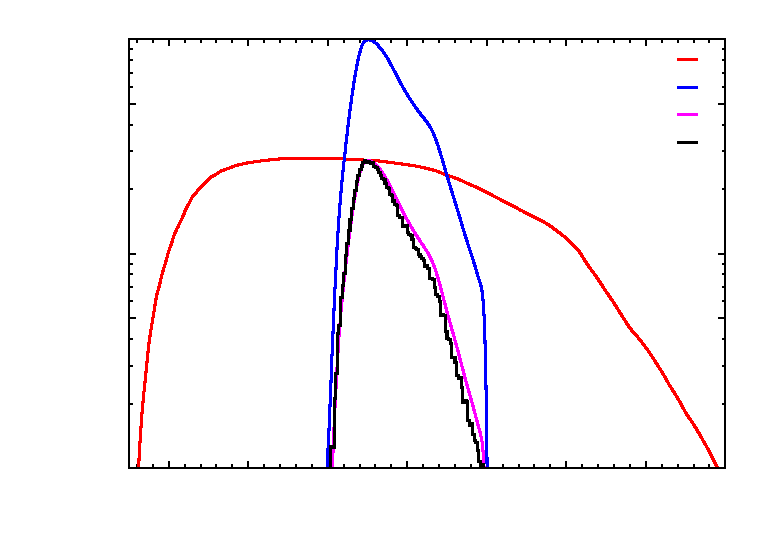
\includegraphics{pics/QE}}%
    \gplfronttext
  \end{picture}%
\endgroup
}
		\captionof{figure}{Plot showing PMT quantum efficiency (red), the scintillator yield (blue), %
			their correlation (magenta) and the distributions of photon collected by the PMT in the GEANT4 %
			simulation of optical photons (black).}
		\label{fig:QE}
	\end{minipage}
\end{figure}

Another possibility as a source for neutron calibration is using californium-252, which %
undergoes $\alpha$ emissions (96.91\%) or spontaneous fission (SF) (3.09\%).
Thanks to a shorter half-life of 2.645\,y, a \tapi{252}Cf source presents a higher activity compared to an Am-Be source %
with the same number of nucleons.
Furthermore, the SF process emits an average of 3.75 neutrons per fission and an average of 10.3 photons %
summing up for a total energy of 8.2\,Mev~\cite{PhysRev.104.699}.
As for the case of the Am-Be calibrating source, the photons can be collected by a scintillating material %
and tag the emission of neutrons.
After the trigger signal, multiple neutron captures on hydrogen are expected, separated by short intervals in time %
of the order of milliseconds.
The yield of multiple neutrons is an advantage that the SNO collaboration exploited to develop a method, %
called \emph{Time Series Analysis}, that uses multiplicity and time intervals between the detected events %
to find the neutron detection efficiency, the neutron mean life inside the detector, %
and activity from non-fission events~\cite{Labranche:2004sya}.
Differently from an Am-Be source, the activity of which must be known precisely, the neutron tagging calibration %
with a californium source can be done in principle regardless of that information.
The fast-neutron and photon energy spectra from \tapi{252}Cf are shown in \ref{fig:spectra}: %
the neutrons are emitted with a most-probable energy of 0.7\,MeV and an average energy of 2.1\,MeV.
It is reasonable to assume that the capture on hydrogen occurs in the proximity of the source, %
bringing about an even more accurate calibration than with the Am-Be source.


We performed some preliminary studies with the aim to develop a device for neutron calibration %
of a generic water Cherenkov detector.
For laboratory measurement, we used a \tapi{252}Cf source with an activity of 4.3\,kBq at the time of its production.
%measured on the 28\tapi{th} of July, 2017.
The californium is encapsulated in a double-hull stainless steel cylinder, 9.5\,mm in diameter and 37.5\,mm high.
The source is placed in a simple prototype of the device, shown in \reffig{fig:setup}, %
consisting of a cylindrical plastic scintillator (EJ-200), coated with mylar to contain optical photons, %
and optically mounted on a ET Enterprise 9902B series~PMT.
A hole, coaxial to the plastic cylinder, allows to insert the source in the middle of the scintillator.
The cylinder is 3\,in in length and 1.5\,in in diameter.
The rate of photons emitted by the \tapi{252}Cf source is measured with this setup; %
the signal from the PMT is amplified and cleaned by NIM modules and finally recorded with a 14-bit VME digitiser.
%to count the number of photon triggers from the PMT and %
%a daisy-chain of NIM amplifier, threshold, and discriminator is used before the digitiser to optimise the signal.
Without the source inside the scintillator, a dark rate of 1.633\,Hz is measured, %
whereas with the source the rate increases to 41.395\,Hz.
The distributions of the PMT peaks collected by the digitiser are shown in Fig.~\ref{fig:source}.
A predicted activity of 3.1\,kBq is expected on the day of the measurement---446 days after the production of the source--- %
which translates to a SF rate of 96.46\,Hz.
The SF tagging efficiency with this setup is therefore estimated to be around~41\,\%.

\begin{figure}
	\begin{minipage}[t]{0.54\textwidth}
		\centering
		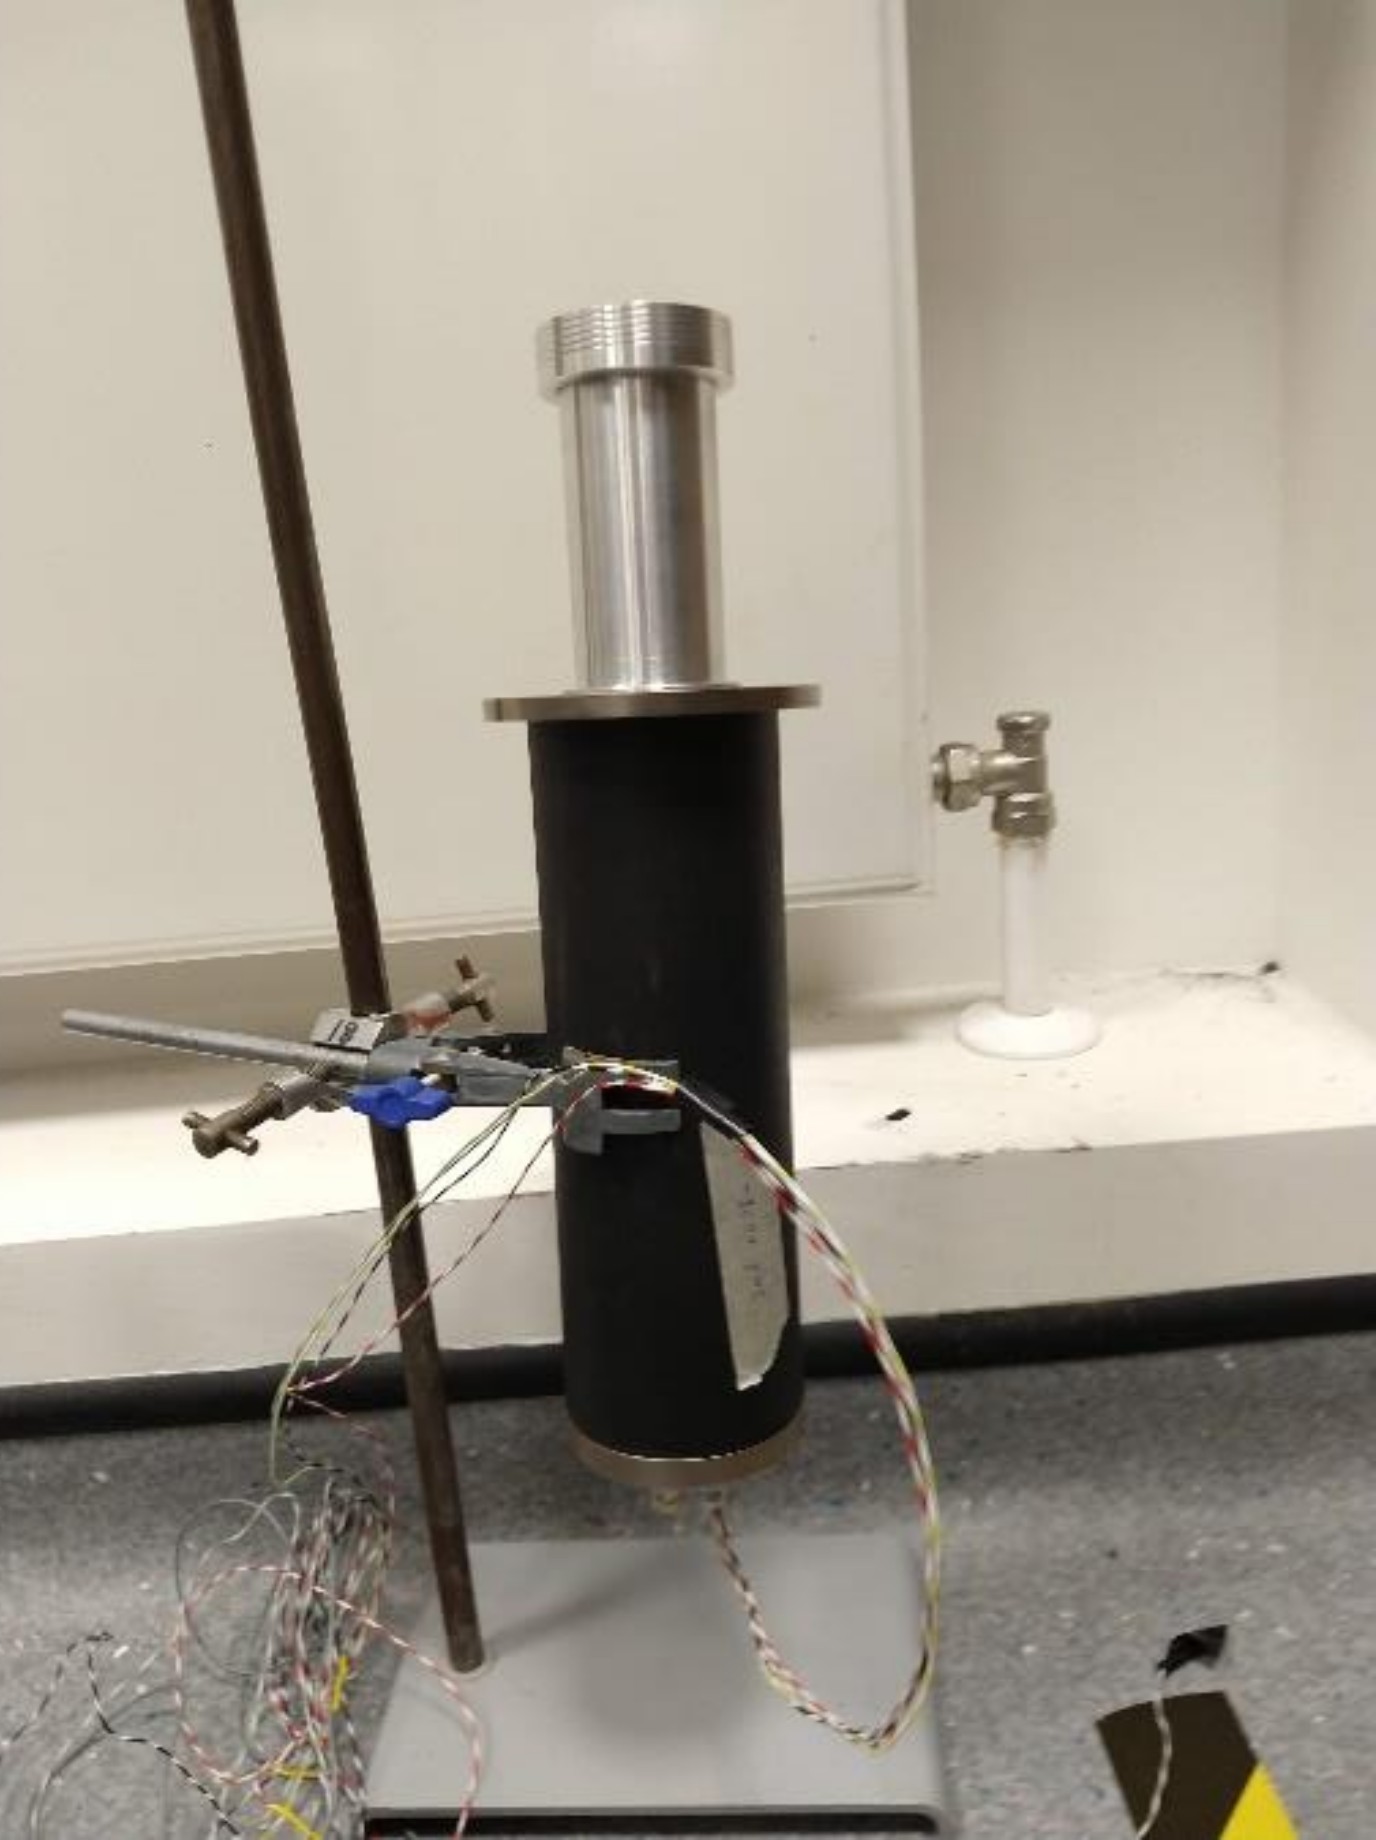
\includegraphics[width=0.4\linewidth]{pics/device.png}
		\raisebox{2.5em}{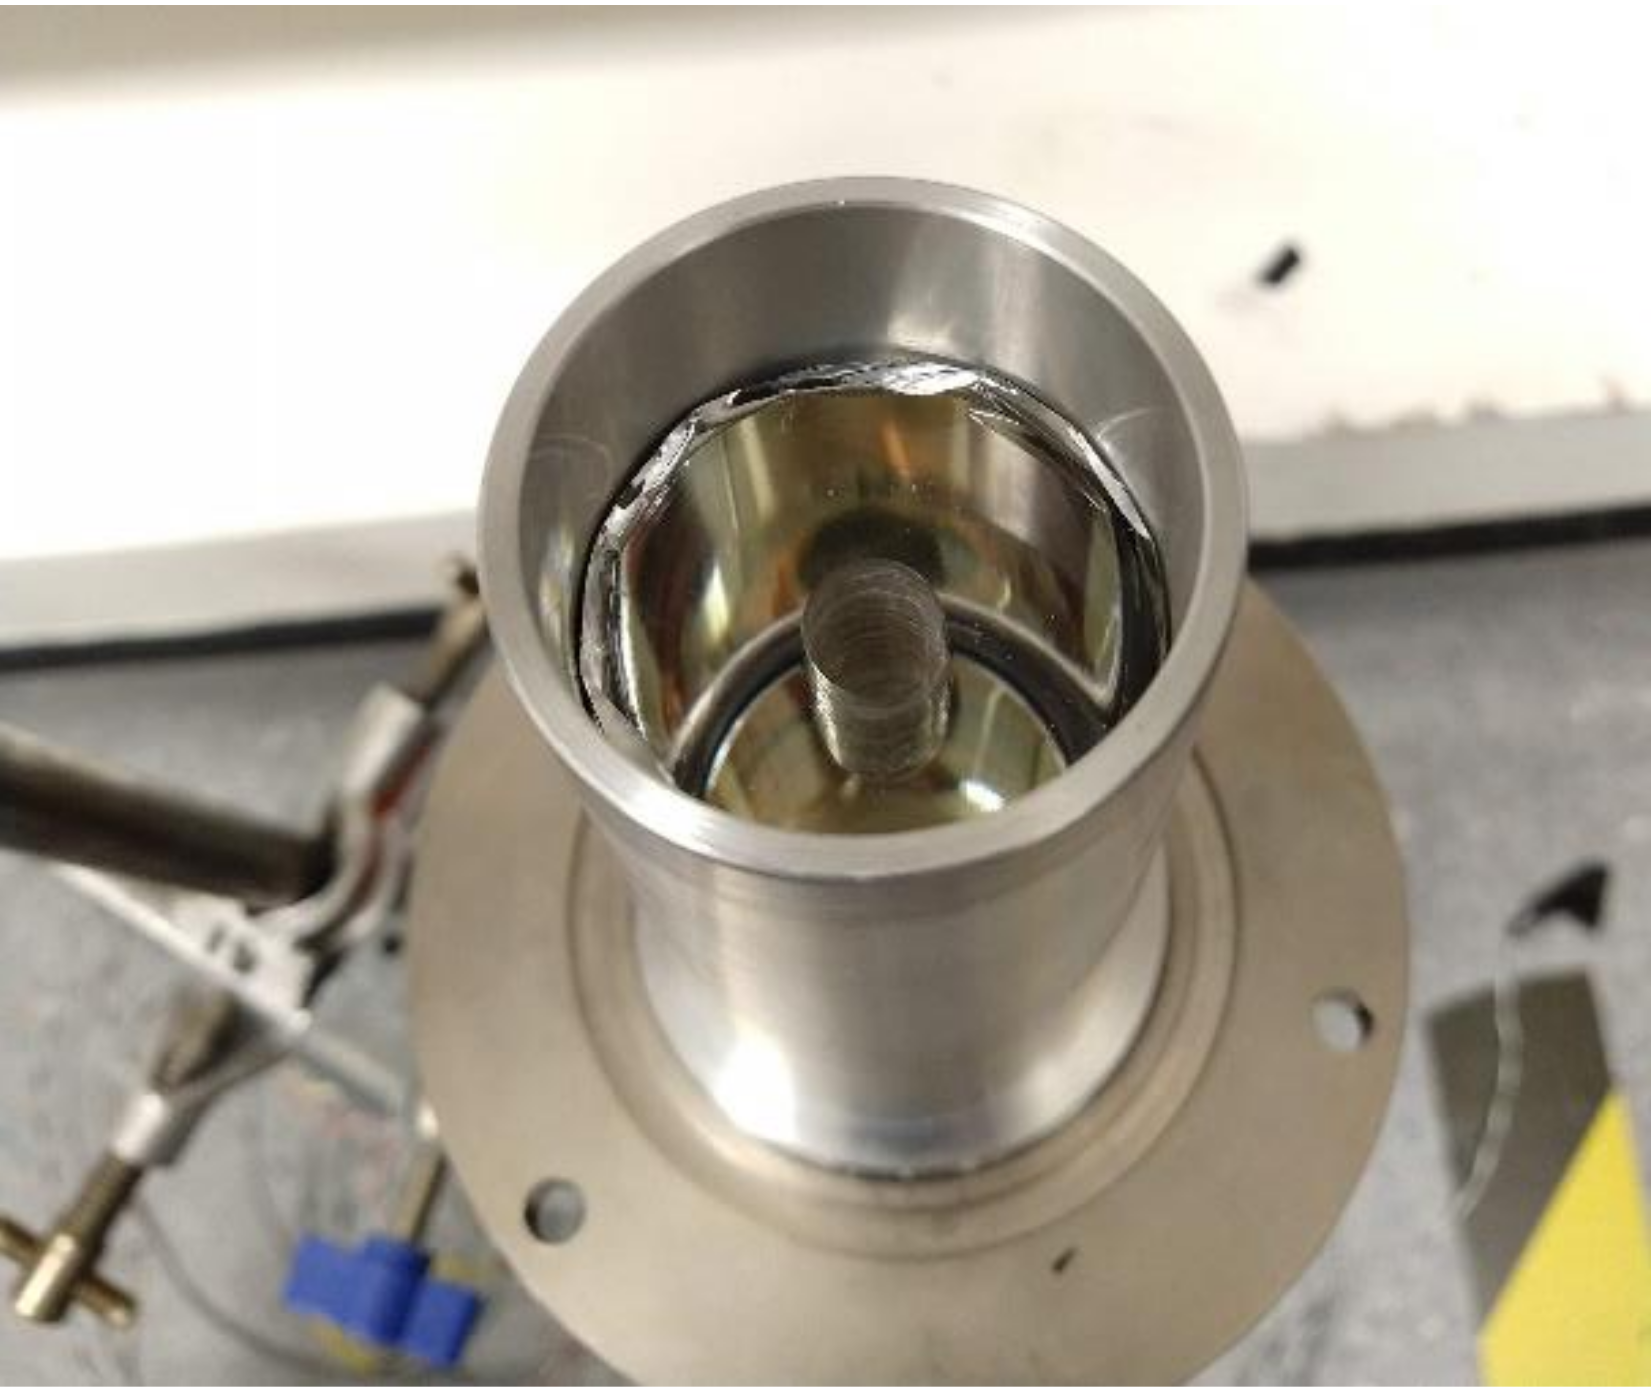
\includegraphics[width=0.4\linewidth]{pics/device_in.png}}
		\captionof{figure}{Setup used to test the californium source.}
		\label{fig:setup}
	\end{minipage}
	\hfill
	\begin{minipage}[t]{0.46\textwidth}
		\centering
		\resizebox{\textwidth}{!}{% GNUPLOT: LaTeX picture with Postscript
\begingroup
  \makeatletter
  \providecommand\color[2][]{%
    \GenericError{(gnuplot) \space\space\space\@spaces}{%
      Package color not loaded in conjunction with
      terminal option `colourtext'%
    }{See the gnuplot documentation for explanation.%
    }{Either use 'blacktext' in gnuplot or load the package
      color.sty in LaTeX.}%
    \renewcommand\color[2][]{}%
  }%
  \providecommand\includegraphics[2][]{%
    \GenericError{(gnuplot) \space\space\space\@spaces}{%
      Package graphicx or graphics not loaded%
    }{See the gnuplot documentation for explanation.%
    }{The gnuplot epslatex terminal needs graphicx.sty or graphics.sty.}%
    \renewcommand\includegraphics[2][]{}%
  }%
  \providecommand\rotatebox[2]{#2}%
  \@ifundefined{ifGPcolor}{%
    \newif\ifGPcolor
    \GPcolortrue
  }{}%
  \@ifundefined{ifGPblacktext}{%
    \newif\ifGPblacktext
    \GPblacktexttrue
  }{}%
  % define a \g@addto@macro without @ in the name:
  \let\gplgaddtomacro\g@addto@macro
  % define empty templates for all commands taking text:
  \gdef\gplbacktext{}%
  \gdef\gplfronttext{}%
  \makeatother
  \ifGPblacktext
    % no textcolor at all
    \def\colorrgb#1{}%
    \def\colorgray#1{}%
  \else
    % gray or color?
    \ifGPcolor
      \def\colorrgb#1{\color[rgb]{#1}}%
      \def\colorgray#1{\color[gray]{#1}}%
      \expandafter\def\csname LTw\endcsname{\color{white}}%
      \expandafter\def\csname LTb\endcsname{\color{black}}%
      \expandafter\def\csname LTa\endcsname{\color{black}}%
      \expandafter\def\csname LT0\endcsname{\color[rgb]{1,0,0}}%
      \expandafter\def\csname LT1\endcsname{\color[rgb]{0,1,0}}%
      \expandafter\def\csname LT2\endcsname{\color[rgb]{0,0,1}}%
      \expandafter\def\csname LT3\endcsname{\color[rgb]{1,0,1}}%
      \expandafter\def\csname LT4\endcsname{\color[rgb]{0,1,1}}%
      \expandafter\def\csname LT5\endcsname{\color[rgb]{1,1,0}}%
      \expandafter\def\csname LT6\endcsname{\color[rgb]{0,0,0}}%
      \expandafter\def\csname LT7\endcsname{\color[rgb]{1,0.3,0}}%
      \expandafter\def\csname LT8\endcsname{\color[rgb]{0.5,0.5,0.5}}%
    \else
      % gray
      \def\colorrgb#1{\color{black}}%
      \def\colorgray#1{\color[gray]{#1}}%
      \expandafter\def\csname LTw\endcsname{\color{white}}%
      \expandafter\def\csname LTb\endcsname{\color{black}}%
      \expandafter\def\csname LTa\endcsname{\color{black}}%
      \expandafter\def\csname LT0\endcsname{\color{black}}%
      \expandafter\def\csname LT1\endcsname{\color{black}}%
      \expandafter\def\csname LT2\endcsname{\color{black}}%
      \expandafter\def\csname LT3\endcsname{\color{black}}%
      \expandafter\def\csname LT4\endcsname{\color{black}}%
      \expandafter\def\csname LT5\endcsname{\color{black}}%
      \expandafter\def\csname LT6\endcsname{\color{black}}%
      \expandafter\def\csname LT7\endcsname{\color{black}}%
      \expandafter\def\csname LT8\endcsname{\color{black}}%
    \fi
  \fi
    \setlength{\unitlength}{0.0500bp}%
    \ifx\gptboxheight\undefined%
      \newlength{\gptboxheight}%
      \newlength{\gptboxwidth}%
      \newsavebox{\gptboxtext}%
    \fi%
    \setlength{\fboxrule}{0.5pt}%
    \setlength{\fboxsep}{1pt}%
\begin{picture}(7200.00,5040.00)%
    \gplgaddtomacro\gplbacktext{%
      \csname LTb\endcsname%%
      \put(1078,704){\makebox(0,0)[r]{\strut{}$10^{-3}$}}%
      \put(1078,1733){\makebox(0,0)[r]{\strut{}$10^{-2}$}}%
      \put(1078,2762){\makebox(0,0)[r]{\strut{}$0.1$}}%
      \put(1078,3790){\makebox(0,0)[r]{\strut{}$1$}}%
      \put(1078,4819){\makebox(0,0)[r]{\strut{}$10$}}%
      \put(1210,484){\makebox(0,0){\strut{}$0$}}%
      \put(2142,484){\makebox(0,0){\strut{}$0.1$}}%
      \put(3074,484){\makebox(0,0){\strut{}$0.2$}}%
      \put(4007,484){\makebox(0,0){\strut{}$0.3$}}%
      \put(4939,484){\makebox(0,0){\strut{}$0.4$}}%
      \put(5871,484){\makebox(0,0){\strut{}$0.5$}}%
      \put(6803,484){\makebox(0,0){\strut{}$0.6$}}%
    }%
    \gplgaddtomacro\gplfronttext{%
      \csname LTb\endcsname%%
      \put(298,2761){\rotatebox{-270}{\makebox(0,0){\strut{}Events / s}}}%
      \put(4006,154){\makebox(0,0){\strut{}Peak (V)}}%
      \csname LTb\endcsname%%
      \put(6212,4624){\makebox(0,0)[r]{\strut{}Source in}}%
      \csname LTb\endcsname%%
      \put(6212,4360){\makebox(0,0)[r]{\strut{}Source out}}%
    }%
    \gplbacktext
    \put(0,0){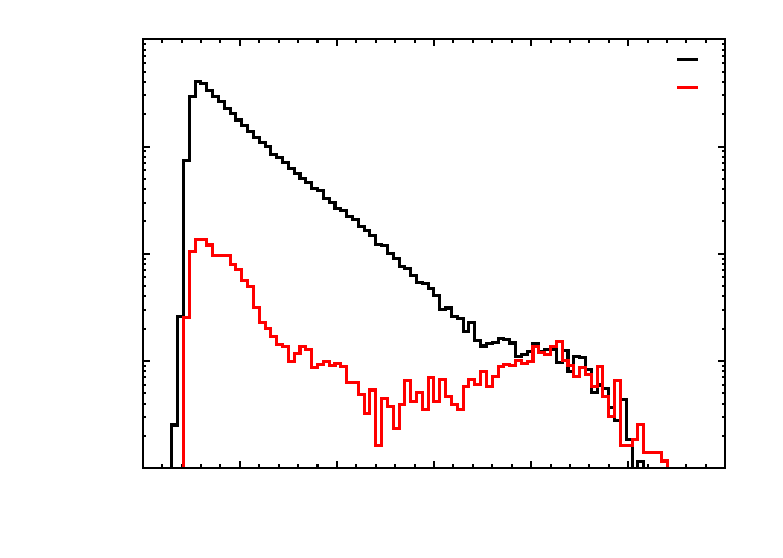
\includegraphics{pics/peaksources}}%
    \gplfronttext
  \end{picture}%
\endgroup
}
		\captionof{figure}{Distribution of PMT peaks measured with source inside (black) and source removed from the scintillator~(red).}
		\label{fig:source}
	\end{minipage}
\end{figure}

We performed a GEANT4~\cite{Agostinelli:2002hh} simulation of the setup, with the aim of optimising the calibration instrument.
An ideal device would absorb all the photons converting them into visible light without affecting the neutrons.
The plot in \reffig{fig:QE} shows the correct implementation of the scintillator and PMT efficiencies in the simulation: %
there is good agreement with the MC distribution and the expected optical photon spectrum.
Different volumes and materials are tested for the scintillator in the simulation.
As materials, BGO crystal and a generic vinyltouluene are chosen.
The selected shapes of the volume are a cube, and cylinder with a diameter-height-ratio 1:1 and 1:2.
The latter shape models the protoype tested in the laboratory.
The characteristic size, i.e.\ the side for the cube and the height for the cylinders, is swept from 1\,cm to 40\,cm.
The simulation tracks the energy deposited in the scintillator by the photons and the number of neutrons escaping the device, %
from a simulation of \np{10000} SF events.
The result is shown in Fig.~\ref{fig:geant4}, where, for both photons and neutrons, %
the average value of the fraction of absorbed energy with respect to the initial one is plotted against the size.
In terms of materials, the BGO crystal unsurprisingly performs better than the plastic scintillator, %
absorbing almost the entirity of photons and leaving the neutrons mainly unaffected.
A part from not being as efficient as scintillator, the hydrogen in the plastic thermalises the neutrons, %
and this might have an impact on the capture time in a water Cherenkov detector.
In terms of sizes and shapes, a BGO cube of $4--6$\,cm sides seems to maximise photon absorption and minimise %
the energy loss of neutrons.
This is in line with the choice for the calibrating device for SK, which is a 5\,cm BGO cube.
Both the cylindrical shapes are optimal when the height is $7\sim11$\,cm, but more crystal would be required %
increasing the cost of the device.
As far as the plastic scintillator is concerned, it is more difficult to define an optimal size/shape figure:
a cubic scintillator is more efficient in collecting photons, but being the form with the largest volume %
per given size, it is also more effective in slowing down neutrons.
The two cylinder shapes have similar performances, proportionally to their volumes.

\begin{figure}
	\centering
	\resizebox{0.9\textwidth}{!}{% GNUPLOT: LaTeX picture with Postscript
\begingroup
  \makeatletter
  \providecommand\color[2][]{%
    \GenericError{(gnuplot) \space\space\space\@spaces}{%
      Package color not loaded in conjunction with
      terminal option `colourtext'%
    }{See the gnuplot documentation for explanation.%
    }{Either use 'blacktext' in gnuplot or load the package
      color.sty in LaTeX.}%
    \renewcommand\color[2][]{}%
  }%
  \providecommand\includegraphics[2][]{%
    \GenericError{(gnuplot) \space\space\space\@spaces}{%
      Package graphicx or graphics not loaded%
    }{See the gnuplot documentation for explanation.%
    }{The gnuplot epslatex terminal needs graphicx.sty or graphics.sty.}%
    \renewcommand\includegraphics[2][]{}%
  }%
  \providecommand\rotatebox[2]{#2}%
  \@ifundefined{ifGPcolor}{%
    \newif\ifGPcolor
    \GPcolortrue
  }{}%
  \@ifundefined{ifGPblacktext}{%
    \newif\ifGPblacktext
    \GPblacktexttrue
  }{}%
  % define a \g@addto@macro without @ in the name:
  \let\gplgaddtomacro\g@addto@macro
  % define empty templates for all commands taking text:
  \gdef\gplbacktext{}%
  \gdef\gplfronttext{}%
  \makeatother
  \ifGPblacktext
    % no textcolor at all
    \def\colorrgb#1{}%
    \def\colorgray#1{}%
  \else
    % gray or color?
    \ifGPcolor
      \def\colorrgb#1{\color[rgb]{#1}}%
      \def\colorgray#1{\color[gray]{#1}}%
      \expandafter\def\csname LTw\endcsname{\color{white}}%
      \expandafter\def\csname LTb\endcsname{\color{black}}%
      \expandafter\def\csname LTa\endcsname{\color{black}}%
      \expandafter\def\csname LT0\endcsname{\color[rgb]{1,0,0}}%
      \expandafter\def\csname LT1\endcsname{\color[rgb]{0,1,0}}%
      \expandafter\def\csname LT2\endcsname{\color[rgb]{0,0,1}}%
      \expandafter\def\csname LT3\endcsname{\color[rgb]{1,0,1}}%
      \expandafter\def\csname LT4\endcsname{\color[rgb]{0,1,1}}%
      \expandafter\def\csname LT5\endcsname{\color[rgb]{1,1,0}}%
      \expandafter\def\csname LT6\endcsname{\color[rgb]{0,0,0}}%
      \expandafter\def\csname LT7\endcsname{\color[rgb]{1,0.3,0}}%
      \expandafter\def\csname LT8\endcsname{\color[rgb]{0.5,0.5,0.5}}%
    \else
      % gray
      \def\colorrgb#1{\color{black}}%
      \def\colorgray#1{\color[gray]{#1}}%
      \expandafter\def\csname LTw\endcsname{\color{white}}%
      \expandafter\def\csname LTb\endcsname{\color{black}}%
      \expandafter\def\csname LTa\endcsname{\color{black}}%
      \expandafter\def\csname LT0\endcsname{\color{black}}%
      \expandafter\def\csname LT1\endcsname{\color{black}}%
      \expandafter\def\csname LT2\endcsname{\color{black}}%
      \expandafter\def\csname LT3\endcsname{\color{black}}%
      \expandafter\def\csname LT4\endcsname{\color{black}}%
      \expandafter\def\csname LT5\endcsname{\color{black}}%
      \expandafter\def\csname LT6\endcsname{\color{black}}%
      \expandafter\def\csname LT7\endcsname{\color{black}}%
      \expandafter\def\csname LT8\endcsname{\color{black}}%
    \fi
  \fi
    \setlength{\unitlength}{0.0500bp}%
    \ifx\gptboxheight\undefined%
      \newlength{\gptboxheight}%
      \newlength{\gptboxwidth}%
      \newsavebox{\gptboxtext}%
    \fi%
    \setlength{\fboxrule}{0.5pt}%
    \setlength{\fboxsep}{1pt}%
\begin{picture}(14400.00,7200.00)%
    \gplgaddtomacro\gplbacktext{%
      \csname LTb\endcsname%%
      \put(618,540){\makebox(0,0)[r]{\strut{}0}}%
      \csname LTb\endcsname%%
      \put(618,1726){\makebox(0,0)[r]{\strut{}0.2}}%
      \csname LTb\endcsname%%
      \put(618,2912){\makebox(0,0)[r]{\strut{}0.4}}%
      \csname LTb\endcsname%%
      \put(618,4098){\makebox(0,0)[r]{\strut{}0.6}}%
      \csname LTb\endcsname%%
      \put(618,5284){\makebox(0,0)[r]{\strut{}0.8}}%
      \csname LTb\endcsname%%
      \put(618,6470){\makebox(0,0)[r]{\strut{}1}}%
      \csname LTb\endcsname%%
      \put(720,354){\makebox(0,0){\strut{}$0$}}%
      \csname LTb\endcsname%%
      \put(1570,354){\makebox(0,0){\strut{}$5$}}%
      \csname LTb\endcsname%%
      \put(2421,354){\makebox(0,0){\strut{}$10$}}%
      \csname LTb\endcsname%%
      \put(3271,354){\makebox(0,0){\strut{}$15$}}%
      \csname LTb\endcsname%%
      \put(4122,354){\makebox(0,0){\strut{}$20$}}%
      \csname LTb\endcsname%%
      \put(4972,354){\makebox(0,0){\strut{}$25$}}%
      \csname LTb\endcsname%%
      \put(5822,354){\makebox(0,0){\strut{}$30$}}%
      \csname LTb\endcsname%%
      \put(6673,354){\makebox(0,0){\strut{}$35$}}%
    }%
    \gplgaddtomacro\gplfronttext{%
      \csname LTb\endcsname%%
      \put(126,3653){\rotatebox{-270}{\makebox(0,0){\strut{}Average fraction of absorbed energy (\%)}}}%
      \csname LTb\endcsname%%
      \put(4121,75){\makebox(0,0){\strut{}Size (cm)}}%
      \csname LTb\endcsname%%
      \put(4121,7046){\makebox(0,0){\strut{}BGO scintillator}}%
      \csname LTb\endcsname%%
      \put(6990,1451){\makebox(0,0)[r]{\strut{}Cube}}%
      \csname LTb\endcsname%%
      \put(6990,1265){\makebox(0,0)[r]{\strut{}Cyl.\ 1:1}}%
      \csname LTb\endcsname%%
      \put(6990,1079){\makebox(0,0)[r]{\strut{}Cyl.\ 1:2}}%
      \csname LTb\endcsname%%
      \put(6990,893){\makebox(0,0)[r]{\strut{}$\gamma$}}%
      \csname LTb\endcsname%%
      \put(6990,707){\makebox(0,0)[r]{\strut{}$n$}}%
    }%
    \gplgaddtomacro\gplbacktext{%
      \csname LTb\endcsname%%
      \put(7421,540){\makebox(0,0)[r]{\strut{}}}%
      \csname LTb\endcsname%%
      \put(7421,1726){\makebox(0,0)[r]{\strut{}}}%
      \csname LTb\endcsname%%
      \put(7421,2912){\makebox(0,0)[r]{\strut{}}}%
      \csname LTb\endcsname%%
      \put(7421,4098){\makebox(0,0)[r]{\strut{}}}%
      \csname LTb\endcsname%%
      \put(7421,5284){\makebox(0,0)[r]{\strut{}}}%
      \csname LTb\endcsname%%
      \put(7421,6470){\makebox(0,0)[r]{\strut{}}}%
      \csname LTb\endcsname%%
      \put(7523,354){\makebox(0,0){\strut{}$0$}}%
      \csname LTb\endcsname%%
      \put(8374,354){\makebox(0,0){\strut{}$5$}}%
      \csname LTb\endcsname%%
      \put(9224,354){\makebox(0,0){\strut{}$10$}}%
      \csname LTb\endcsname%%
      \put(10075,354){\makebox(0,0){\strut{}$15$}}%
      \csname LTb\endcsname%%
      \put(10925,354){\makebox(0,0){\strut{}$20$}}%
      \csname LTb\endcsname%%
      \put(11776,354){\makebox(0,0){\strut{}$25$}}%
      \csname LTb\endcsname%%
      \put(12626,354){\makebox(0,0){\strut{}$30$}}%
      \csname LTb\endcsname%%
      \put(13477,354){\makebox(0,0){\strut{}$35$}}%
      \csname LTb\endcsname%%
      \put(14327,354){\makebox(0,0){\strut{}$40$}}%
    }%
    \gplgaddtomacro\gplfronttext{%
      \csname LTb\endcsname%%
      \put(10925,75){\makebox(0,0){\strut{}Size (cm)}}%
      \csname LTb\endcsname%%
      \put(10925,7046){\makebox(0,0){\strut{}Plastic scintillator}}%
      \csname LTb\endcsname%%
      \put(13794,1451){\makebox(0,0)[r]{\strut{}Cube}}%
      \csname LTb\endcsname%%
      \put(13794,1265){\makebox(0,0)[r]{\strut{}Cyl.\ 1:1}}%
      \csname LTb\endcsname%%
      \put(13794,1079){\makebox(0,0)[r]{\strut{}Cyl.\ 1:2}}%
      \csname LTb\endcsname%%
      \put(13794,893){\makebox(0,0)[r]{\strut{}$\gamma$}}%
      \csname LTb\endcsname%%
      \put(13794,707){\makebox(0,0)[r]{\strut{}$n$}}%
    }%
    \gplbacktext
    \put(0,0){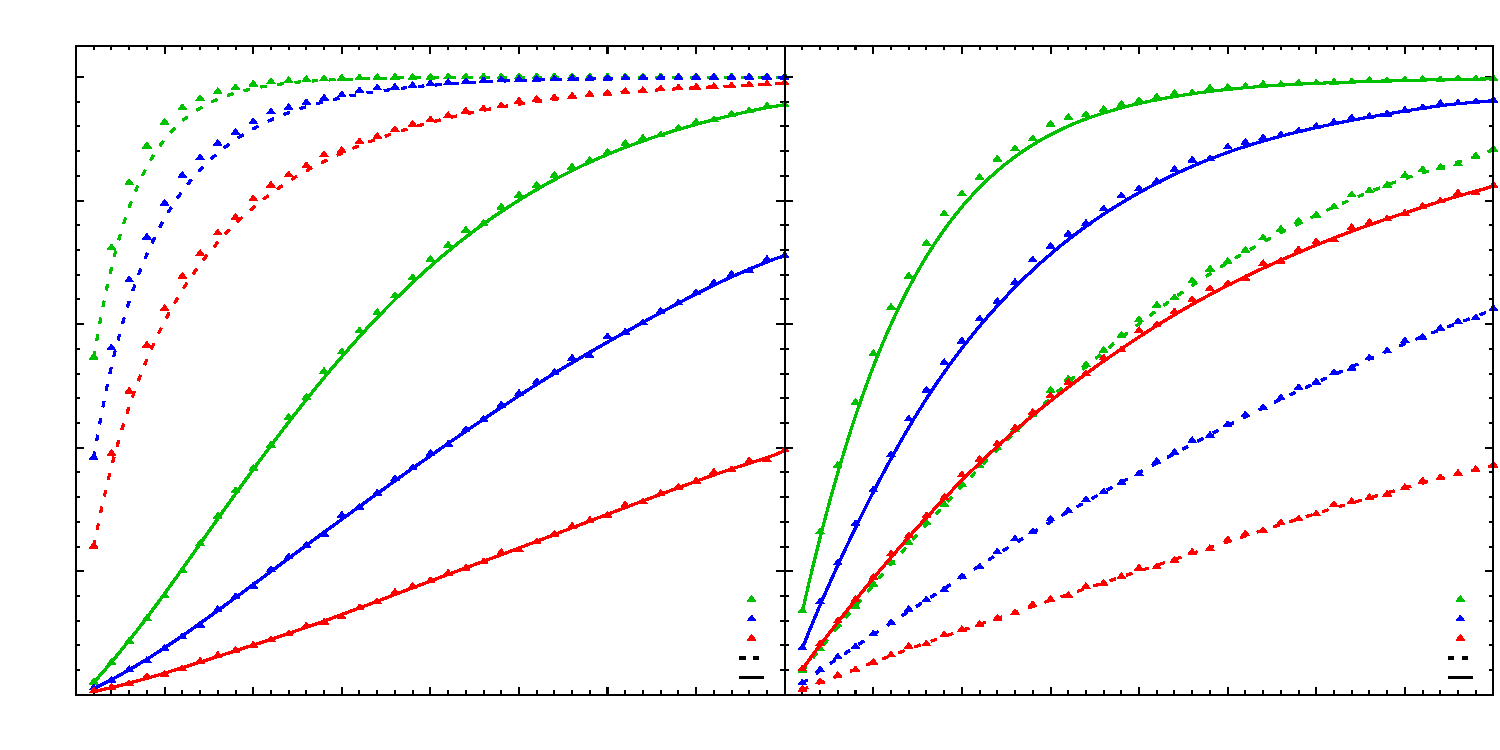
\includegraphics{n_vs_gamma_2}}%
    \gplfronttext
  \end{picture}%
\endgroup
}
	\caption{Result of the GEANT4 simulation, showing the performance of different scintillators.
		The fraction of absorbed energy per initial energy of neutrons (solid) and photons (dashed) %
		is averaged and plotted against the scintillator size.
		Three shapes are tested: a cube (green), a cylinder with diameter-height-ratio of 1:1 (blue), %
		and a cylinder with ratio 1:2 (red).
		On the left, the scintillating material is BGO crystal; on the right, %
		a generic vinyltouluene plastic is used.}
	\label{fig:geant4}
\end{figure}


%To verify neutron tagging efficiency given above, experimental tests were conducted with an Am/Be source embedded in a bismuth germanite (BGO) scintillator. The prompt and delayed event-pair is generated via: α + 9Be →12
%C∗+n; 12C∗ →12 C+γ(prompt); n+p → d+γ(delayed).
%The scintillation light induced by 4.43 MeV deexcitation γ
%serves as the primary event. Note that the reaction to the
%ground state of 12C also exists, where no 4.43 MeV deexcitation γ is emitted. The experimental apparatus was
%deployed at the center of the tank, during which the trigger
%gate to catch 2.2 MeV γ was temporarily enlarged to 800
%μs in order to obtain a complete neutron capture time spectrum. To estimate source related background (e.g. ground
%transition neutron), 10 Hz 800μs random trigger data was
%also taken.
%The final N10 distribution after all cuts applied is shown in
%Fig. 2, where for Am/Be data all backgrounds are subtracted according to random trigger data. Signal efficiencies for
%MC and data are (19.2±0.1)% and (19.0±0.2)%, respectively. Data is in good agreement with MC. Fig. 3 shows
%the distribution of time difference (ΔT) between delayed
%neutron signal and prompt event. The neutron lifetime in
%pure water is measured to be (201.8 ± 4.7)μs using a unbinned maximum likelihood fitting as shown in Fig. 3.
%
%The Am-Be source is embedded in a 5 cm cube of BGO scintillator (see figure 8.27)
%to amplify the light released by the 4.4 MeV γ-ray, such that it will activate the SHE
%trigger in the detector. Upon triggering SHE stores 35µs of data, and then an extended
%AFT trigger is activated to store an additional 800µs, and grant a more complete view
%the neutron capture time spectrum.
%Figure 8.27: Am-Be crystal embedded in a 5 cm cube of BGO scintillator. This is
%held in an acrylic case.
%This configuration was set up in 3 different locations around the tank: the centre (35.3,
%-70.7, 0) cm (Centre), near the side of the barrel (35.3, -1201.9, 0) cm (Y12), and near
%the top of the tank (35.3, -70.7, 1500.0) cm (Z15). Random data was also taken with
%the apparatus in the centre, using a 10Hz trigger, to study the irreducible background
%from the ground-state transition.
%
%
%Neutron tagging is then performed on the remaining Am-Be dataset, and a 2.2 MeV
%γ-ray MC. There are some differences between this study and the atmospheric neutrino study discussed up until now. Neutrons released by Beryllium have an energy
%ranging from 2-10 MeV, much less than the average neutron energy following atmospheric neutrino interactions. Thus, we can make the assumption that the location of
%the Am-Be apparatus is roughly the same as the neutron capture vertex. This raises
%the expected neutron detection efficiency in accordance with figure 8.23. In addition,
%Chapter 8. Neutron Tagging 140
%the PMT after-pulse observed following high energy atmospheric neutrino events (figure 8.5) is not produced to the same extent after Am-Be events, so neutron searching
%is started at 5µs (previously > 18µs) after the primary trigger. The AFT trigger for
%Am-Be is also extended, allowing neutron-searching until 835µs after the initial trigger.
%The efficiency is calculated by fitting the timing distribution of neutron candidates to a
%constant background + exponentially decaying signal representing the neutron capture
%lifetime.


\section{Gadolinium neutron capture}
\label{sec:gadolinium}

%In the next phase of the Super-Kamiokande experiment, a gadolinium salt compound Gd\tped{2}(SO\tped{4})\tped{3} %
%will be added to the detector~\cite{}, which will improve the ability of the detector to identify neutrons.
%Neutrons are emitted in inverse beta decay (IBD) process, $\cj{\nu}_e + p \to e^+ + n$.
%The current technique to tag neutrons in SK is by detecting capture on hydrogen nuclei.
%Capture of a thermal neutron on hydrogen has a cross-section of $\np{332.6}\pm\np{0.7}$~\,b, %
%characteristic time of $\sim200$\,\textmu s in water, with the release of $\np{2.2}$\,MeV gammas.
%After the prompt Cherenkov radiation from the charged lepton, the secondary signal from an electron, %
%compton-scattered by the 2.2\,MeV photon, is looked for in a long time window.
%However, in water what matters are the electrons Compton-scattered above the Cerenkov threshold by relatively hard gammas.
%
%The detectable light following neutron capture on Gd (in thin foils) in possible discrete counters was carefully simulated %
%for the SNO heavy water Cerenkov detector.
%The equivalent single electron energy was found to peak at about 5 MeV, and range over 3--8\,MeV.
%This spread reflects the intrinsic variation in the gamma cascades and the detector energy
%resolution (the simulation had 5 photoelectrons per MeV of electron energy, compared to 6 in SK-I)~\cite{Beacom:2003nk}.
%The energy threshold for SK is 5\,MeV, and the search of hydrogen-tagged neutrons is not efficient (20\%).
%a long time window in which to look for the hydrogen signal, 
%Capture on gadolinium has a cross-section of $\np{49e3}$~b, which de-excites emitting a $\sim\np{8}$~MeV gamma-ray cascade.
%By adding 0.2\,\% by mass of the Gd salt as Gd\tped{2}(SO\tped{4})\tped{3}, the characteristic time of capture is %
%$\sim30$~\textmu s and an efficiency of 90\,\% can be achieved.
%The isotopes \tapi{155}Gd and \tapi{157}Gd present very high cross-sections to thermal neutron capture, %
%respectively \np{6.074e4}\,b and \np{2.537e5}\,b.
%Hydrogen alone has a cross-section of \np{3.321e-1}\,b.


Gadolinium-157 has the highest thermal neutron capture cross-section among any stable nuclides.
It is estimated to be \np{2.537E5}\,b, but the natural abundance of \tapi{157}Gd is around 15.65\,\%.
Another isotope of gadolinium with similar abundance is \tapi{155}Gd, at 14.80\,\%, %
which also presents a very high neutron capture cross-section \np{6.074E4}\,b.
Dissolving gadolinium compounds in water could therefore considerably increase the neutron capture %
probability, as proposed for the first time in \refref{Beacom:2003nk}.
Gd-doped water enhances the capture cross-section, with an effective cross-section of \np{49e3}\,b, %
compared to pure water with $\sim$0.3\,b on a free proton.
Upon capturing a neutron, the Gd emits three to four gamma rays having a total energy of about 8\,MeV.
Such energetic photons can produce Cherenkov light via Compton-scattering and therefore they can be 
reliably detected in a large detector volume.
The neutron in gadolinium-loaded water thermalises quicker than in just pure water, with a %
characteristic time of $\sim$30\,\textmu s, and it can be captured by a Gd nucleus with an %
estimated efficiency of 90\,\%~\cite{Beacom:2003nk} for a 0.2\,\% Gd solution (see \reffig{fig:gd_conc}).
%The time and spatial correlation of the positron and neutron capture events ($20~\mu$s and 4~cm) %
%can significantly reduce the backgrounds, and hence enhance the nu e signal events.
%Even moderately energetic neutrons ranging from tens to hundreds of MeV will quickly lose energy %
%by collisions with free protons and oxygen nuclei in water. 
%Once thermalised, the neutrons undergo radiative capture, combining with a nearby nucleus to %
%produce a more tightly bound final state, with excess energy released in a gamma-ray ( ) cascade. 

%\iffalse
\begin{figure}
	\begin{minipage}[t]{0.48\textwidth}
		\centering
		\resizebox{0.9\linewidth}{!}{% GNUPLOT: LaTeX picture with Postscript
\begingroup
  \makeatletter
  \providecommand\color[2][]{%
    \GenericError{(gnuplot) \space\space\space\@spaces}{%
      Package color not loaded in conjunction with
      terminal option `colourtext'%
    }{See the gnuplot documentation for explanation.%
    }{Either use 'blacktext' in gnuplot or load the package
      color.sty in LaTeX.}%
    \renewcommand\color[2][]{}%
  }%
  \providecommand\includegraphics[2][]{%
    \GenericError{(gnuplot) \space\space\space\@spaces}{%
      Package graphicx or graphics not loaded%
    }{See the gnuplot documentation for explanation.%
    }{The gnuplot epslatex terminal needs graphicx.sty or graphics.sty.}%
    \renewcommand\includegraphics[2][]{}%
  }%
  \providecommand\rotatebox[2]{#2}%
  \@ifundefined{ifGPcolor}{%
    \newif\ifGPcolor
    \GPcolortrue
  }{}%
  \@ifundefined{ifGPblacktext}{%
    \newif\ifGPblacktext
    \GPblacktexttrue
  }{}%
  % define a \g@addto@macro without @ in the name:
  \let\gplgaddtomacro\g@addto@macro
  % define empty templates for all commands taking text:
  \gdef\gplbacktext{}%
  \gdef\gplfronttext{}%
  \makeatother
  \ifGPblacktext
    % no textcolor at all
    \def\colorrgb#1{}%
    \def\colorgray#1{}%
  \else
    % gray or color?
    \ifGPcolor
      \def\colorrgb#1{\color[rgb]{#1}}%
      \def\colorgray#1{\color[gray]{#1}}%
      \expandafter\def\csname LTw\endcsname{\color{white}}%
      \expandafter\def\csname LTb\endcsname{\color{black}}%
      \expandafter\def\csname LTa\endcsname{\color{black}}%
      \expandafter\def\csname LT0\endcsname{\color[rgb]{1,0,0}}%
      \expandafter\def\csname LT1\endcsname{\color[rgb]{0,1,0}}%
      \expandafter\def\csname LT2\endcsname{\color[rgb]{0,0,1}}%
      \expandafter\def\csname LT3\endcsname{\color[rgb]{1,0,1}}%
      \expandafter\def\csname LT4\endcsname{\color[rgb]{0,1,1}}%
      \expandafter\def\csname LT5\endcsname{\color[rgb]{1,1,0}}%
      \expandafter\def\csname LT6\endcsname{\color[rgb]{0,0,0}}%
      \expandafter\def\csname LT7\endcsname{\color[rgb]{1,0.3,0}}%
      \expandafter\def\csname LT8\endcsname{\color[rgb]{0.5,0.5,0.5}}%
    \else
      % gray
      \def\colorrgb#1{\color{black}}%
      \def\colorgray#1{\color[gray]{#1}}%
      \expandafter\def\csname LTw\endcsname{\color{white}}%
      \expandafter\def\csname LTb\endcsname{\color{black}}%
      \expandafter\def\csname LTa\endcsname{\color{black}}%
      \expandafter\def\csname LT0\endcsname{\color{black}}%
      \expandafter\def\csname LT1\endcsname{\color{black}}%
      \expandafter\def\csname LT2\endcsname{\color{black}}%
      \expandafter\def\csname LT3\endcsname{\color{black}}%
      \expandafter\def\csname LT4\endcsname{\color{black}}%
      \expandafter\def\csname LT5\endcsname{\color{black}}%
      \expandafter\def\csname LT6\endcsname{\color{black}}%
      \expandafter\def\csname LT7\endcsname{\color{black}}%
      \expandafter\def\csname LT8\endcsname{\color{black}}%
    \fi
  \fi
    \setlength{\unitlength}{0.0500bp}%
    \ifx\gptboxheight\undefined%
      \newlength{\gptboxheight}%
      \newlength{\gptboxwidth}%
      \newsavebox{\gptboxtext}%
    \fi%
    \setlength{\fboxrule}{0.5pt}%
    \setlength{\fboxsep}{1pt}%
\begin{picture}(7200.00,5040.00)%
    \gplgaddtomacro\gplbacktext{%
      \csname LTb\endcsname%%
      \put(645,595){\makebox(0,0)[r]{\strut{}$0$}}%
      \csname LTb\endcsname%%
      \put(645,1465){\makebox(0,0)[r]{\strut{}$20$}}%
      \csname LTb\endcsname%%
      \put(645,2335){\makebox(0,0)[r]{\strut{}$40$}}%
      \csname LTb\endcsname%%
      \put(645,3206){\makebox(0,0)[r]{\strut{}$60$}}%
      \csname LTb\endcsname%%
      \put(645,4076){\makebox(0,0)[r]{\strut{}$80$}}%
      \csname LTb\endcsname%%
      \put(645,4946){\makebox(0,0)[r]{\strut{}$100$}}%
      \csname LTb\endcsname%%
      \put(747,409){\makebox(0,0){\strut{}$0.0001$}}%
      \csname LTb\endcsname%%
      \put(2347,409){\makebox(0,0){\strut{}$0.001$}}%
      \csname LTb\endcsname%%
      \put(3948,409){\makebox(0,0){\strut{}$0.01$}}%
      \csname LTb\endcsname%%
      \put(5548,409){\makebox(0,0){\strut{}$0.1$}}%
      \csname LTb\endcsname%%
      \put(7148,409){\makebox(0,0){\strut{}$1$}}%
      \csname LTb\endcsname%%
      \put(4229,4076){\makebox(0,0)[r]{\strut{}0.02\,\%}}%
      \csname LTb\endcsname%%
      \put(5830,3206){\makebox(0,0)[r]{\strut{}0.2\,\%}}%
    }%
    \gplgaddtomacro\gplfronttext{%
      \csname LTb\endcsname%%
      \put(153,2770){\rotatebox{-270}{\makebox(0,0){\strut{}Capture efficiency (\%)}}}%
      \csname LTb\endcsname%%
      \put(3947,130){\makebox(0,0){\strut{}Gd concentration (\%)}}%
    }%
    \gplbacktext
    \put(0,0){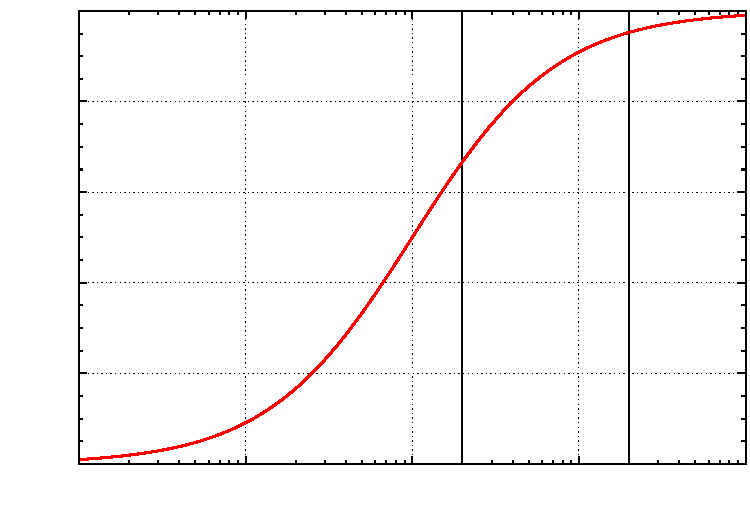
\includegraphics{pics/gdconcentration}}%
    \gplfronttext
  \end{picture}%
\endgroup
}
		\captionof{figure}{Estimated dependency of neutron capture efficiency on gadolinium with respect to the gadolinium %
			concentration in water. Super-Kamiokande will start with a 0.02\,\% Gd-load, %
			increasing up to 0.2\,\% to reach an expected $\sim$90\,\% capture efficiency.}
		\label{fig:gd_conc}
	\end{minipage}
	\hfill
	\begin{minipage}[t]{0.5\textwidth}
		\centering
		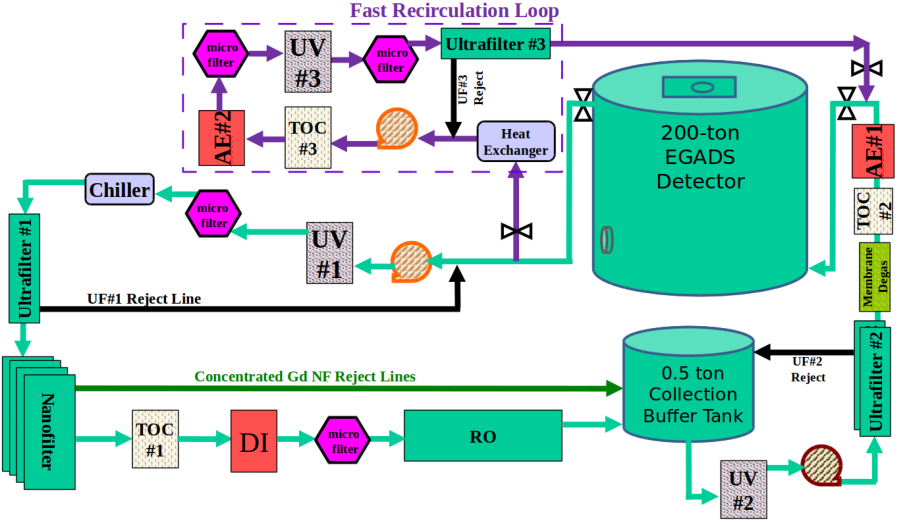
\includegraphics[width=\linewidth]{pics/bandpass.pdf}
		\captionof{figure}{Schematic of the band-pass filtration system and the fast recirculation loop, %
			where the main components of the system are highlighted: anion-exchange resins (AE), %
			ultraviolet lamp (UV), total organic compung lamp (TOC), deionising system (DI), %
			reverse osmosis stage (RO). See text and \refref{Ikeda:2019pcm} for details. }
		\label{fig:egads}
	\end{minipage}
\end{figure}
%\fi

\iffalse
\begin{figure}
	\centering
	\resizebox{0.5\linewidth}{!}{% GNUPLOT: LaTeX picture with Postscript
\begingroup
  \makeatletter
  \providecommand\color[2][]{%
    \GenericError{(gnuplot) \space\space\space\@spaces}{%
      Package color not loaded in conjunction with
      terminal option `colourtext'%
    }{See the gnuplot documentation for explanation.%
    }{Either use 'blacktext' in gnuplot or load the package
      color.sty in LaTeX.}%
    \renewcommand\color[2][]{}%
  }%
  \providecommand\includegraphics[2][]{%
    \GenericError{(gnuplot) \space\space\space\@spaces}{%
      Package graphicx or graphics not loaded%
    }{See the gnuplot documentation for explanation.%
    }{The gnuplot epslatex terminal needs graphicx.sty or graphics.sty.}%
    \renewcommand\includegraphics[2][]{}%
  }%
  \providecommand\rotatebox[2]{#2}%
  \@ifundefined{ifGPcolor}{%
    \newif\ifGPcolor
    \GPcolortrue
  }{}%
  \@ifundefined{ifGPblacktext}{%
    \newif\ifGPblacktext
    \GPblacktexttrue
  }{}%
  % define a \g@addto@macro without @ in the name:
  \let\gplgaddtomacro\g@addto@macro
  % define empty templates for all commands taking text:
  \gdef\gplbacktext{}%
  \gdef\gplfronttext{}%
  \makeatother
  \ifGPblacktext
    % no textcolor at all
    \def\colorrgb#1{}%
    \def\colorgray#1{}%
  \else
    % gray or color?
    \ifGPcolor
      \def\colorrgb#1{\color[rgb]{#1}}%
      \def\colorgray#1{\color[gray]{#1}}%
      \expandafter\def\csname LTw\endcsname{\color{white}}%
      \expandafter\def\csname LTb\endcsname{\color{black}}%
      \expandafter\def\csname LTa\endcsname{\color{black}}%
      \expandafter\def\csname LT0\endcsname{\color[rgb]{1,0,0}}%
      \expandafter\def\csname LT1\endcsname{\color[rgb]{0,1,0}}%
      \expandafter\def\csname LT2\endcsname{\color[rgb]{0,0,1}}%
      \expandafter\def\csname LT3\endcsname{\color[rgb]{1,0,1}}%
      \expandafter\def\csname LT4\endcsname{\color[rgb]{0,1,1}}%
      \expandafter\def\csname LT5\endcsname{\color[rgb]{1,1,0}}%
      \expandafter\def\csname LT6\endcsname{\color[rgb]{0,0,0}}%
      \expandafter\def\csname LT7\endcsname{\color[rgb]{1,0.3,0}}%
      \expandafter\def\csname LT8\endcsname{\color[rgb]{0.5,0.5,0.5}}%
    \else
      % gray
      \def\colorrgb#1{\color{black}}%
      \def\colorgray#1{\color[gray]{#1}}%
      \expandafter\def\csname LTw\endcsname{\color{white}}%
      \expandafter\def\csname LTb\endcsname{\color{black}}%
      \expandafter\def\csname LTa\endcsname{\color{black}}%
      \expandafter\def\csname LT0\endcsname{\color{black}}%
      \expandafter\def\csname LT1\endcsname{\color{black}}%
      \expandafter\def\csname LT2\endcsname{\color{black}}%
      \expandafter\def\csname LT3\endcsname{\color{black}}%
      \expandafter\def\csname LT4\endcsname{\color{black}}%
      \expandafter\def\csname LT5\endcsname{\color{black}}%
      \expandafter\def\csname LT6\endcsname{\color{black}}%
      \expandafter\def\csname LT7\endcsname{\color{black}}%
      \expandafter\def\csname LT8\endcsname{\color{black}}%
    \fi
  \fi
    \setlength{\unitlength}{0.0500bp}%
    \ifx\gptboxheight\undefined%
      \newlength{\gptboxheight}%
      \newlength{\gptboxwidth}%
      \newsavebox{\gptboxtext}%
    \fi%
    \setlength{\fboxrule}{0.5pt}%
    \setlength{\fboxsep}{1pt}%
\begin{picture}(7200.00,5040.00)%
    \gplgaddtomacro\gplbacktext{%
      \csname LTb\endcsname%%
      \put(645,595){\makebox(0,0)[r]{\strut{}$0$}}%
      \csname LTb\endcsname%%
      \put(645,1465){\makebox(0,0)[r]{\strut{}$20$}}%
      \csname LTb\endcsname%%
      \put(645,2335){\makebox(0,0)[r]{\strut{}$40$}}%
      \csname LTb\endcsname%%
      \put(645,3206){\makebox(0,0)[r]{\strut{}$60$}}%
      \csname LTb\endcsname%%
      \put(645,4076){\makebox(0,0)[r]{\strut{}$80$}}%
      \csname LTb\endcsname%%
      \put(645,4946){\makebox(0,0)[r]{\strut{}$100$}}%
      \csname LTb\endcsname%%
      \put(747,409){\makebox(0,0){\strut{}$0.0001$}}%
      \csname LTb\endcsname%%
      \put(2347,409){\makebox(0,0){\strut{}$0.001$}}%
      \csname LTb\endcsname%%
      \put(3948,409){\makebox(0,0){\strut{}$0.01$}}%
      \csname LTb\endcsname%%
      \put(5548,409){\makebox(0,0){\strut{}$0.1$}}%
      \csname LTb\endcsname%%
      \put(7148,409){\makebox(0,0){\strut{}$1$}}%
      \csname LTb\endcsname%%
      \put(4229,4076){\makebox(0,0)[r]{\strut{}0.02\,\%}}%
      \csname LTb\endcsname%%
      \put(5830,3206){\makebox(0,0)[r]{\strut{}0.2\,\%}}%
    }%
    \gplgaddtomacro\gplfronttext{%
      \csname LTb\endcsname%%
      \put(153,2770){\rotatebox{-270}{\makebox(0,0){\strut{}Capture efficiency (\%)}}}%
      \csname LTb\endcsname%%
      \put(3947,130){\makebox(0,0){\strut{}Gd concentration (\%)}}%
    }%
    \gplbacktext
    \put(0,0){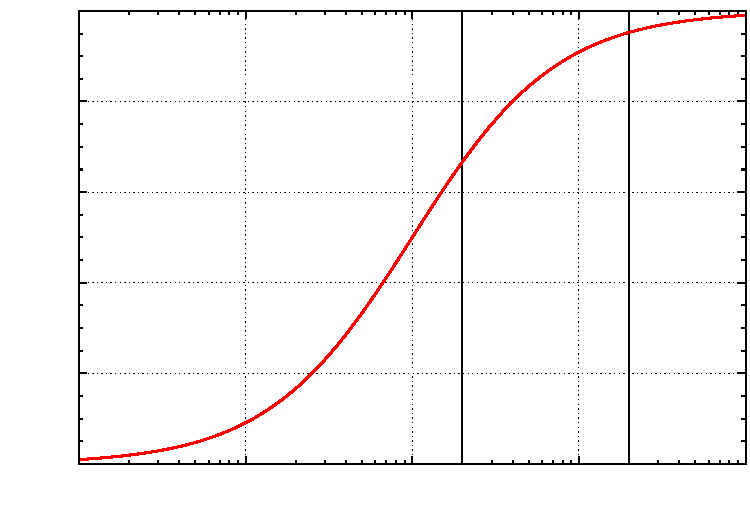
\includegraphics{pics/gdconcentration}}%
    \gplfronttext
  \end{picture}%
\endgroup
}
	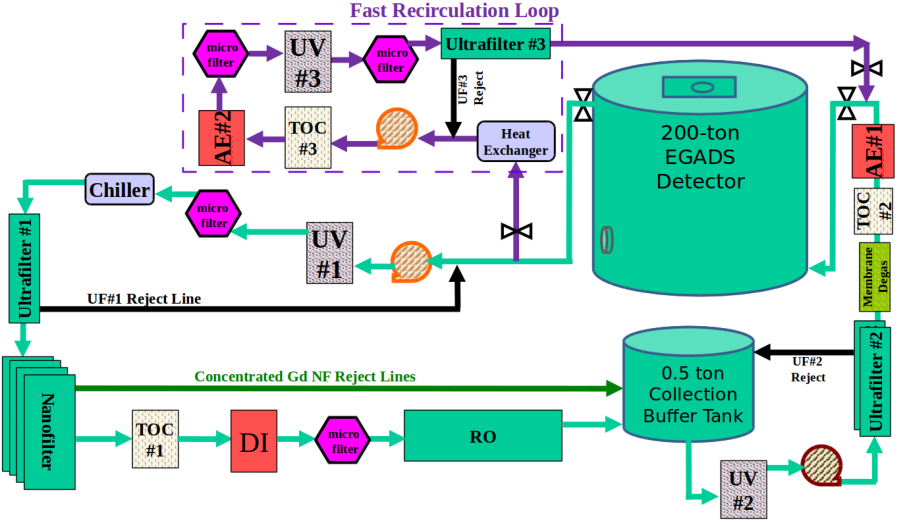
\includegraphics[width=0.45\textwidth]{pics/bandpass.pdf}
	\caption{Estimated dependency of neutron capture efficiency on gadolinium with respect to the gadolinium %
		concentration in water. Super-Kamiokande will start with a 0.02\,\% Gd-load, %
		increasing up to 0.2\,\% to reach an expected $\sim$90\,\% capture efficiency.}
	\label{fig:gd_conc}
\end{figure}
\fi


In the next phase of the Super-Kamiokande experiment, a gadolinium salt compound %
will be dissolved in the detector to improve the ability to identify neutrons.
This is possible thanks to extensive R\&D performed with the EGADS experiment~\cite{Ikeda:2019pcm}.
In \refref{Beacom:2003nk}, gadolinium trichloride GdCl\tped{3} was proposed, %
but the current full-scale plan for SK and EGADS has setteled on using gadolinium sulfate Gd\tped{2}(SO\tped{4})\tped{3}.
%---another candidate being 
This choice was determined by a few requirements by which a Gd compound canditate must comply.
In addition to the aforementioned salts, a third option could have been gadolinium nitrate Gd(NO\tped{3})\tped{3}).
The candidate compound must be water soluble, also in large amounts, but all of the three gadolinium salts %
easily dissolve in water.
%The above three candidates can all be dissolved fairly easily, with the GdCl3 and Gd(NO3)3 only
%needing stirring to fully dissolve, while the Gd2(SO4)3, can be forced into solution with the addition of %
%a small amount of sulfuric acid, about 380 ml of acid for 28 kg of Gd2(SO4)3 in 14 tons of water (test done at EGADS).
%So, this solubility requirement does not immediately rule out any of these three compounds.
If used in very large quantities, as it will be for SK, the compund must be safe for %
%Next, if the compound is to be used inside a very large water Cherenkov detector, such as SK, it must be safe for
the detectors components and it should be non-toxical. %it may be easily put into existing detectors.
None of the above salts are toxic, but GdCl\tped{3} is corrosive and not suitable for a full scale test.
Soak tests in a Gd solution at $25^\circ$C showed that the rubber friction pads used to hold the ID PMT %
is susceptible to the sulfate, even though they seem to be affected also by pure water.
In over twenty years of operation of SK, the effect has never been noticed, meaning the filtration system %
removes the impurities from this material with great success.
Taking in account the different scales of the detector and the test and that the typical temperature %
of the water in SK is around $13^\circ$C, the case was deemed not to be a potential problem.
%they show different corrosive properties, due to the different anions of the molecule.
%The nitrate and the sulfate turn out to be non-corrosive, and do not seem to affect detectors components much, if at all.
%An extensive soak test study was carried out in Japan, with each of the 31 different materials inside the SK detector %
%being soaked in both pure water and Gd2(SO4)3 solution.
%Only the which it is in the case of SK.
%However, the chloride is corrosive, so for this reason the GdCl3 has been ruled out as a full scale test candidate.
It is also necessary that the gadolinium solution maintains a high level of optical transparency, %
so that optical photons of Cherenkov radiation can propagate inside the tank without attenuation.
The Gd(NO\tped{3})\tped{3} is opaque in the UV region of the electromagnetic spectrum, for wavelengths less than 350\,nm, %
and this unfortunately is where a large fraction of Cherenkov light is detected in SK PMTs, %
so it cannot be a good full scale test candidate either.
This leaves Gd2(SO4)3 as the only choice possible, having good transparency in the UV and optical regions.
%This is in fact the choice that has been made by the EGADS group, and the remaining studies described in this paper %
%have been done using, or under the assumption that, Gd2(SO4)3 will be used.
%One last exceptionally nice quality about this compound is today it costs only 5 US dollars per kilogram, %
%meaning it would only be about 500,000 US dollars to dope SK, a price which is on the scale of such a major %
%experiment~\cite{1201.1017}[conference].

The most challenging aspect of a gadolinium-loaded water Cherenkov detector is the filtration system.
The SK water purification system produces ultrapure water, close to the theoretical maximum, %
with a resistivity around $18$\,M$\Omega\cdot$cm.
This high purity is achieved thanks to several filtration stages, including microfilters, %
ultrafilters (less than 0.1\,\textmu m), UV lamps for bacterial growth, reverse osmosis,  vacuum and membrane degasifiers, and anion-exchange resins.
The current process, without modifications, would completely remove dissolved gadolinium.
Therefore, in order to keep good water quality and high transparency, it is necessary to adapt the purification system %
such that it can remove all impurities, ions included, except Gd\tapi{3+} and its anionic partner (SO\tped{4})\tapi{2-}.
A new filtration system, called ``band-pass filtration system'', has been devised for EGADS and runs in parallel to %
the fast-recirculation loop~\cite{Ikeda:2019pcm}.
The schematic is illustrated in \reffig{fig:egads}.
The water from the water Cherenkov tank is first cleaned by microfilters and UV light.
The Gd solution is then cooled down, as the sulfate dissolves better at lower temperatures, %
before passing through an ultafilter.
At this stage, a series of nanofilters splits up the water line into Gd-enriched water and %
water with less than one part-per-milion of gadolinium.
The concentrated line goes directly back to a buffer collection tank, whereas the gadolinium-free line %
is first cleaned by deionisation and reverse osmosis.
In the collection tank, dissolved air is removed by a membrane degassifier and resins are used %
for the final purification.
After full loading up to a concentration of 0.2\,\% of Gd, the water transparency is found to within typical SK values %
thanks to the water filtration system which can maintain good water quality and minimises gadolinium losses.

The water system for the gadolinium phase of SK will be essentially a scaled version of the EGADS filtration system.
During the first stage, a solution of 0.02\,\% in Gd\tped{2}(SO\tped{4})\tped{3} mass will be loaded in SK, %
to progressively increase it up to 0.2\,\% after the first comissioning.

\section{Monitoring gadolinium concentration}
\label{sec:gad}

The concentration of Gd in water affects the efficiency and timing of neutron captures, %
which must be known for an accurate measurement of antineutrino rate.
It is fundamental, therefore, to measure the concentration regularly, as this can change in time inside the detector.
On large scales like for SK, it is not a trivial task to predict the temperature and the flow dependency %
of the dissolved Gd.
At the moment, the EGADS experiment keeps track of the Gd concentration with a Zeeman atomic absorption spectrometer (AAS), %
located near the experiment.
Water samples are collected monthly from the water tank, diluted and atomised inside the AAS machine.
The amount of Gd is then compared to known samples of Gd loaded water to determine the concentration.

We propose an alternative method for monitoring gadolinium concentration, %
which still uses atomic absorption lines of Gd, but in solution in water.
Gadolinium presents strong emission/absorption lines in the UV region~\cite{Morton_2000}.
Using a UV source and a spectrometer it is possible to measure the absorption by gadolinium dissolved in water.
The absorbance in directly proportional to the amount of gadolinium and therefore to the concentration, %
where absorbance is defined as
\begin{equation}
	\mathcal{A}(x) = \log_{10} \frac{I_0 (x)}{I_\text{Gd}(x)}\ .
\end{equation}
The spectrum $I_0$ of a reference sample of pure water is taken before the gadolinium loaded water sample $I_\text{Gd}$.
These two spectrum are then compared at a given wavelength.
The gadolinium absorbance spectrum presents a series of lines in the 270\,nm -- 275\,nm region.
The height of one peak is related to the concentration, as the amount of light surviving the sample is related to
\begin{equation}
	I_\text{Gd}(x) = I_0(x) e^{-\flatfrac{\ell}{\lambda}}\ ,
\end{equation}
with $\lambda$ the attenuantion length and $\ell$ the sample length.
For a fixed cross-section volume and a fixed-length sample, the attenuation length will %
decrease with the amount of Gd in the sample $m_\text{Gd}$, or since the volume is constant, with the concentration of Gd $\rho_\text{Gd}$.
\begin{equation}
	\rho_\text{Gd} = \frac{m_\text{Gd}}{X\,\ell}\ .
\end{equation}
The Beer-Lambert law relates the optical attenuation of a physical material containing a single attenuating species %
of uniform concentration to the optical path length through the sample and absorptivity of the species.
\begin{equation}
	\mathcal{A} = \varepsilon\, \ell\, \rho = \log_{10} (e) \frac{\ell}{\lambda}\ ,
\end{equation}
where $\varepsilon$ is the molar attenuation coefficient, or absorptivity, of the attenuating species.
The Beer-Lambert law agrees with the expectation of decreasing attenuation length with increasing concentration.


\begin{figure}
	\centering
	\resizebox{0.45\linewidth}{!}{% GNUPLOT: LaTeX picture with Postscript
\begingroup
  \makeatletter
  \providecommand\color[2][]{%
    \GenericError{(gnuplot) \space\space\space\@spaces}{%
      Package color not loaded in conjunction with
      terminal option `colourtext'%
    }{See the gnuplot documentation for explanation.%
    }{Either use 'blacktext' in gnuplot or load the package
      color.sty in LaTeX.}%
    \renewcommand\color[2][]{}%
  }%
  \providecommand\includegraphics[2][]{%
    \GenericError{(gnuplot) \space\space\space\@spaces}{%
      Package graphicx or graphics not loaded%
    }{See the gnuplot documentation for explanation.%
    }{The gnuplot epslatex terminal needs graphicx.sty or graphics.sty.}%
    \renewcommand\includegraphics[2][]{}%
  }%
  \providecommand\rotatebox[2]{#2}%
  \@ifundefined{ifGPcolor}{%
    \newif\ifGPcolor
    \GPcolortrue
  }{}%
  \@ifundefined{ifGPblacktext}{%
    \newif\ifGPblacktext
    \GPblacktexttrue
  }{}%
  % define a \g@addto@macro without @ in the name:
  \let\gplgaddtomacro\g@addto@macro
  % define empty templates for all commands taking text:
  \gdef\gplbacktext{}%
  \gdef\gplfronttext{}%
  \makeatother
  \ifGPblacktext
    % no textcolor at all
    \def\colorrgb#1{}%
    \def\colorgray#1{}%
  \else
    % gray or color?
    \ifGPcolor
      \def\colorrgb#1{\color[rgb]{#1}}%
      \def\colorgray#1{\color[gray]{#1}}%
      \expandafter\def\csname LTw\endcsname{\color{white}}%
      \expandafter\def\csname LTb\endcsname{\color{black}}%
      \expandafter\def\csname LTa\endcsname{\color{black}}%
      \expandafter\def\csname LT0\endcsname{\color[rgb]{1,0,0}}%
      \expandafter\def\csname LT1\endcsname{\color[rgb]{0,1,0}}%
      \expandafter\def\csname LT2\endcsname{\color[rgb]{0,0,1}}%
      \expandafter\def\csname LT3\endcsname{\color[rgb]{1,0,1}}%
      \expandafter\def\csname LT4\endcsname{\color[rgb]{0,1,1}}%
      \expandafter\def\csname LT5\endcsname{\color[rgb]{1,1,0}}%
      \expandafter\def\csname LT6\endcsname{\color[rgb]{0,0,0}}%
      \expandafter\def\csname LT7\endcsname{\color[rgb]{1,0.3,0}}%
      \expandafter\def\csname LT8\endcsname{\color[rgb]{0.5,0.5,0.5}}%
    \else
      % gray
      \def\colorrgb#1{\color{black}}%
      \def\colorgray#1{\color[gray]{#1}}%
      \expandafter\def\csname LTw\endcsname{\color{white}}%
      \expandafter\def\csname LTb\endcsname{\color{black}}%
      \expandafter\def\csname LTa\endcsname{\color{black}}%
      \expandafter\def\csname LT0\endcsname{\color{black}}%
      \expandafter\def\csname LT1\endcsname{\color{black}}%
      \expandafter\def\csname LT2\endcsname{\color{black}}%
      \expandafter\def\csname LT3\endcsname{\color{black}}%
      \expandafter\def\csname LT4\endcsname{\color{black}}%
      \expandafter\def\csname LT5\endcsname{\color{black}}%
      \expandafter\def\csname LT6\endcsname{\color{black}}%
      \expandafter\def\csname LT7\endcsname{\color{black}}%
      \expandafter\def\csname LT8\endcsname{\color{black}}%
    \fi
  \fi
    \setlength{\unitlength}{0.0500bp}%
    \ifx\gptboxheight\undefined%
      \newlength{\gptboxheight}%
      \newlength{\gptboxwidth}%
      \newsavebox{\gptboxtext}%
    \fi%
    \setlength{\fboxrule}{0.5pt}%
    \setlength{\fboxsep}{1pt}%
\begin{picture}(7200.00,5040.00)%
    \gplgaddtomacro\gplbacktext{%
      \csname LTb\endcsname%%
      \put(951,595){\makebox(0,0)[r]{\strut{}$-0.002$}}%
      \csname LTb\endcsname%%
      \put(951,1447){\makebox(0,0)[r]{\strut{}$0.002$}}%
      \csname LTb\endcsname%%
      \put(951,2298){\makebox(0,0)[r]{\strut{}$0.006$}}%
      \csname LTb\endcsname%%
      \put(951,3150){\makebox(0,0)[r]{\strut{}$0.01$}}%
      \csname LTb\endcsname%%
      \put(951,4001){\makebox(0,0)[r]{\strut{}$0.014$}}%
      \csname LTb\endcsname%%
      \put(951,4853){\makebox(0,0)[r]{\strut{}$0.018$}}%
      \csname LTb\endcsname%%
      \put(1053,409){\makebox(0,0){\strut{}$265$}}%
      \csname LTb\endcsname%%
      \put(1628,409){\makebox(0,0){\strut{}$267$}}%
      \csname LTb\endcsname%%
      \put(2202,409){\makebox(0,0){\strut{}$269$}}%
      \csname LTb\endcsname%%
      \put(2777,409){\makebox(0,0){\strut{}$271$}}%
      \csname LTb\endcsname%%
      \put(3352,409){\makebox(0,0){\strut{}$273$}}%
      \csname LTb\endcsname%%
      \put(3927,409){\makebox(0,0){\strut{}$275$}}%
      \csname LTb\endcsname%%
      \put(4501,409){\makebox(0,0){\strut{}$277$}}%
      \csname LTb\endcsname%%
      \put(5076,409){\makebox(0,0){\strut{}$279$}}%
      \csname LTb\endcsname%%
      \put(5651,409){\makebox(0,0){\strut{}$281$}}%
      \csname LTb\endcsname%%
      \put(6225,409){\makebox(0,0){\strut{}$283$}}%
      \csname LTb\endcsname%%
      \put(6800,409){\makebox(0,0){\strut{}$285$}}%
      \csname LTb\endcsname%%
      \put(3064,4001){\makebox(0,0)[r]{\strut{}peak \#1}}%
      \csname LTb\endcsname%%
      \put(4214,3150){\makebox(0,0)[l]{\strut{}peak \#2}}%
    }%
    \gplgaddtomacro\gplfronttext{%
      \csname LTb\endcsname%%
      \put(153,2724){\rotatebox{-270}{\makebox(0,0){\strut{}Abosrbance / 1 cm}}}%
      \csname LTb\endcsname%%
      \put(7004,2724){\rotatebox{-270}{\makebox(0,0){\strut{}}}}%
      \csname LTb\endcsname%%
      \put(3926,130){\makebox(0,0){\strut{}Wavelength (nm)}}%
      \csname LTb\endcsname%%
      \put(3926,4760){\makebox(0,0){\strut{}}}%
      \csname LTb\endcsname%%
      \put(3926,4853){\makebox(0,0){\strut{}}}%
      \csname LTb\endcsname%%
      \put(6355,4686){\makebox(0,0){\strut{}}}%
    }%
    \gplbacktext
    \put(0,0){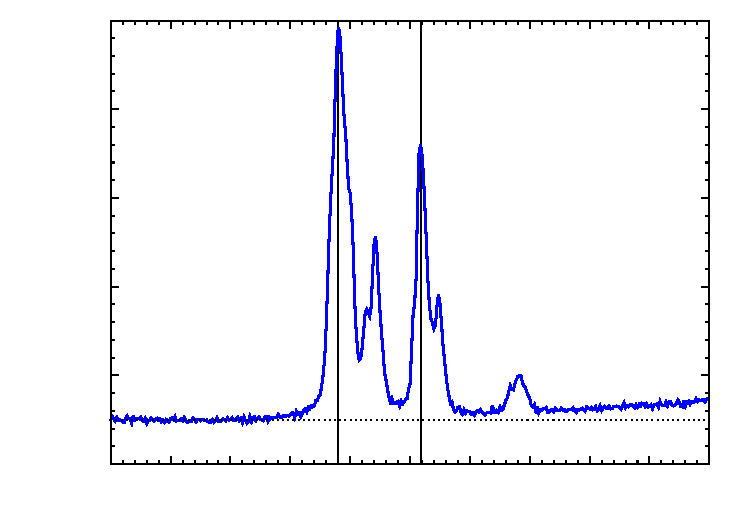
\includegraphics{pics/shimadzu_20}}%
    \gplfronttext
  \end{picture}%
\endgroup
}
	\resizebox{0.45\linewidth}{!}{% GNUPLOT: LaTeX picture with Postscript
\begingroup
  \makeatletter
  \providecommand\color[2][]{%
    \GenericError{(gnuplot) \space\space\space\@spaces}{%
      Package color not loaded in conjunction with
      terminal option `colourtext'%
    }{See the gnuplot documentation for explanation.%
    }{Either use 'blacktext' in gnuplot or load the package
      color.sty in LaTeX.}%
    \renewcommand\color[2][]{}%
  }%
  \providecommand\includegraphics[2][]{%
    \GenericError{(gnuplot) \space\space\space\@spaces}{%
      Package graphicx or graphics not loaded%
    }{See the gnuplot documentation for explanation.%
    }{The gnuplot epslatex terminal needs graphicx.sty or graphics.sty.}%
    \renewcommand\includegraphics[2][]{}%
  }%
  \providecommand\rotatebox[2]{#2}%
  \@ifundefined{ifGPcolor}{%
    \newif\ifGPcolor
    \GPcolortrue
  }{}%
  \@ifundefined{ifGPblacktext}{%
    \newif\ifGPblacktext
    \GPblacktexttrue
  }{}%
  % define a \g@addto@macro without @ in the name:
  \let\gplgaddtomacro\g@addto@macro
  % define empty templates for all commands taking text:
  \gdef\gplbacktext{}%
  \gdef\gplfronttext{}%
  \makeatother
  \ifGPblacktext
    % no textcolor at all
    \def\colorrgb#1{}%
    \def\colorgray#1{}%
  \else
    % gray or color?
    \ifGPcolor
      \def\colorrgb#1{\color[rgb]{#1}}%
      \def\colorgray#1{\color[gray]{#1}}%
      \expandafter\def\csname LTw\endcsname{\color{white}}%
      \expandafter\def\csname LTb\endcsname{\color{black}}%
      \expandafter\def\csname LTa\endcsname{\color{black}}%
      \expandafter\def\csname LT0\endcsname{\color[rgb]{1,0,0}}%
      \expandafter\def\csname LT1\endcsname{\color[rgb]{0,1,0}}%
      \expandafter\def\csname LT2\endcsname{\color[rgb]{0,0,1}}%
      \expandafter\def\csname LT3\endcsname{\color[rgb]{1,0,1}}%
      \expandafter\def\csname LT4\endcsname{\color[rgb]{0,1,1}}%
      \expandafter\def\csname LT5\endcsname{\color[rgb]{1,1,0}}%
      \expandafter\def\csname LT6\endcsname{\color[rgb]{0,0,0}}%
      \expandafter\def\csname LT7\endcsname{\color[rgb]{1,0.3,0}}%
      \expandafter\def\csname LT8\endcsname{\color[rgb]{0.5,0.5,0.5}}%
    \else
      % gray
      \def\colorrgb#1{\color{black}}%
      \def\colorgray#1{\color[gray]{#1}}%
      \expandafter\def\csname LTw\endcsname{\color{white}}%
      \expandafter\def\csname LTb\endcsname{\color{black}}%
      \expandafter\def\csname LTa\endcsname{\color{black}}%
      \expandafter\def\csname LT0\endcsname{\color{black}}%
      \expandafter\def\csname LT1\endcsname{\color{black}}%
      \expandafter\def\csname LT2\endcsname{\color{black}}%
      \expandafter\def\csname LT3\endcsname{\color{black}}%
      \expandafter\def\csname LT4\endcsname{\color{black}}%
      \expandafter\def\csname LT5\endcsname{\color{black}}%
      \expandafter\def\csname LT6\endcsname{\color{black}}%
      \expandafter\def\csname LT7\endcsname{\color{black}}%
      \expandafter\def\csname LT8\endcsname{\color{black}}%
    \fi
  \fi
    \setlength{\unitlength}{0.0500bp}%
    \ifx\gptboxheight\undefined%
      \newlength{\gptboxheight}%
      \newlength{\gptboxwidth}%
      \newsavebox{\gptboxtext}%
    \fi%
    \setlength{\fboxrule}{0.5pt}%
    \setlength{\fboxsep}{1pt}%
\begin{picture}(7200.00,5040.00)%
    \gplgaddtomacro\gplbacktext{%
      \csname LTb\endcsname%%
      \put(951,595){\makebox(0,0)[r]{\strut{}$-0.002$}}%
      \csname LTb\endcsname%%
      \put(951,1305){\makebox(0,0)[r]{\strut{}$0$}}%
      \csname LTb\endcsname%%
      \put(951,2014){\makebox(0,0)[r]{\strut{}$0.002$}}%
      \csname LTb\endcsname%%
      \put(951,2724){\makebox(0,0)[r]{\strut{}$0.004$}}%
      \csname LTb\endcsname%%
      \put(951,3434){\makebox(0,0)[r]{\strut{}$0.006$}}%
      \csname LTb\endcsname%%
      \put(951,4143){\makebox(0,0)[r]{\strut{}$0.008$}}%
      \csname LTb\endcsname%%
      \put(951,4853){\makebox(0,0)[r]{\strut{}$0.01$}}%
      \csname LTb\endcsname%%
      \put(1053,409){\makebox(0,0){\strut{}$265$}}%
      \csname LTb\endcsname%%
      \put(1637,409){\makebox(0,0){\strut{}$267$}}%
      \csname LTb\endcsname%%
      \put(2221,409){\makebox(0,0){\strut{}$269$}}%
      \csname LTb\endcsname%%
      \put(2805,409){\makebox(0,0){\strut{}$271$}}%
      \csname LTb\endcsname%%
      \put(3389,409){\makebox(0,0){\strut{}$273$}}%
      \csname LTb\endcsname%%
      \put(3973,409){\makebox(0,0){\strut{}$275$}}%
      \csname LTb\endcsname%%
      \put(4557,409){\makebox(0,0){\strut{}$277$}}%
      \csname LTb\endcsname%%
      \put(5141,409){\makebox(0,0){\strut{}$279$}}%
      \csname LTb\endcsname%%
      \put(5725,409){\makebox(0,0){\strut{}$281$}}%
      \csname LTb\endcsname%%
      \put(6309,409){\makebox(0,0){\strut{}$283$}}%
      \csname LTb\endcsname%%
      \put(6893,409){\makebox(0,0){\strut{}$285$}}%
      \csname LTb\endcsname%%
      \put(3097,4143){\makebox(0,0)[r]{\strut{}peak \#1}}%
      \csname LTb\endcsname%%
      \put(4265,3079){\makebox(0,0)[l]{\strut{}peak \#2}}%
    }%
    \gplgaddtomacro\gplfronttext{%
      \csname LTb\endcsname%%
      \put(153,2724){\rotatebox{-270}{\makebox(0,0){\strut{}Absorbance / 1\,cm}}}%
      \csname LTb\endcsname%%
      \put(3973,130){\makebox(0,0){\strut{}Wavelength (nm)}}%
      \csname LTb\endcsname%%
      \put(5975,4686){\makebox(0,0)[l]{\strut{}0.2032\%}}%
      \csname LTb\endcsname%%
      \put(5975,4500){\makebox(0,0)[l]{\strut{}0.1847\%}}%
      \csname LTb\endcsname%%
      \put(5975,4314){\makebox(0,0)[l]{\strut{}0.1693\%}}%
      \csname LTb\endcsname%%
      \put(5975,4128){\makebox(0,0)[l]{\strut{}0.1563\%}}%
      \csname LTb\endcsname%%
      \put(5975,3942){\makebox(0,0)[l]{\strut{}0.1451\%}}%
      \csname LTb\endcsname%%
      \put(5975,3756){\makebox(0,0)[l]{\strut{}0.1355\%}}%
      \csname LTb\endcsname%%
      \put(5975,3570){\makebox(0,0)[l]{\strut{}0.1270\%}}%
      \csname LTb\endcsname%%
      \put(5975,3384){\makebox(0,0)[l]{\strut{}0.1195\%}}%
      \csname LTb\endcsname%%
      \put(5975,3198){\makebox(0,0)[l]{\strut{}0.1129\%}}%
      \csname LTb\endcsname%%
      \put(5975,3012){\makebox(0,0)[l]{\strut{}0.1070\%}}%
      \csname LTb\endcsname%%
      \put(5975,2826){\makebox(0,0)[l]{\strut{}0.1016\%}}%
      \csname LTb\endcsname%%
      \put(5975,2640){\makebox(0,0)[l]{\strut{}0.0200\%}}%
    }%
    \gplbacktext
    \put(0,0){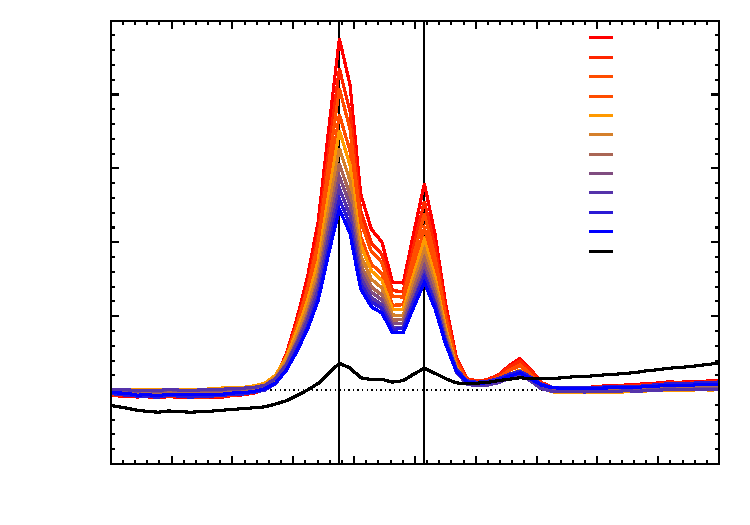
\includegraphics{pics/hdxabs}}%
    \gplfronttext
  \end{picture}%
\endgroup
}
	\caption{Gadolinium absorption lines. }
	\label{fig:gad_lines}
\end{figure}


In an absorbance measurement, however, there could be other sources of absorption.
In a real setup, a light source and a photo sensor are needed, in addition to optical interfaces with the %
sample to measure; the solvent of the sample will also contribute to the overall absorbance.
The Beer-Lamber law can be generalised to a generic $N$ number of attenuating elements
\begin{equation}
	\mathcal{A} = \sum_{i = 1}^N \varepsilon_i \int_0^\ell \dd{z} \rho_i (x) = %
	\varepsilon \ell \rho_0 +  \sum_{i = 1}^{N-1} \varepsilon_i \int_0^\ell \dd{z} \rho_i (x) = a + b \, \rho_0\ ,
\end{equation}
where the attenuating species of interest has been isolated: %
if the other elements are constant, there is a linear law with measured absorbance and concentration.
The absorbance will also depend on the solvent, \ie water, purity and other factors, \eg optical interfaces etc.
The measurement of absorption could also be biased by the presence of wavelength-independent factors, %
or at least independent in the portion of the spectrum of interest.
Examples of these factors could are micro-bubbles or other impurities in the samples.
Micro-bubbles will scatter or block light, thus adding a bias on teh absorbance measurement.
Using two absorption peaks the measurement could be improved by taking the difference of the absorption, %
as any effect which is wavelength independent is removed.
\begin{equation}
	\Delta \mathcal{A} = \mathcal{A}(x_1) - \mathcal{A}(x_2) = %
	\log_{10} \frac{I_0 (x_1)}{I(x_1)} - \log_{10} \frac{I_0 (x_2)}{I(x_2)}\ .
\end{equation}
Supposing the intensity of the reference sample is reduced by a factor $\eta$, %
whereas the intensity of the study sample is reduced by a factor $\zeta$, we would have
\begin{equation}
	\Delta \mathcal{A} = %
	\log_{10} \frac{\eta I_0 (x_1)}{\zeta I(x_1)} - \log_{10} \frac{\eta I_0 (x_2)}{\zeta I(x_2)} = %
	\log_{10} \frac{I_0 (x_1)}{I(x_1)} - \log_{10} \frac{I_0 (x_2)}{I(x_2)}\ ,
\end{equation}
since the difference of two logarithmic elements is taken.
The drawback of this method is that two measurements are needed at the two wavelengths $x_1$ and $x_2$, %
and therefore the error on the measurement will increase by a factor $\sim \sqrt{2}$.

\begin{figure}
	\centering
	\resizebox{0.8\linewidth}{!}{% GNUPLOT: LaTeX picture with Postscript
\begingroup
  \makeatletter
  \providecommand\color[2][]{%
    \GenericError{(gnuplot) \space\space\space\@spaces}{%
      Package color not loaded in conjunction with
      terminal option `colourtext'%
    }{See the gnuplot documentation for explanation.%
    }{Either use 'blacktext' in gnuplot or load the package
      color.sty in LaTeX.}%
    \renewcommand\color[2][]{}%
  }%
  \providecommand\includegraphics[2][]{%
    \GenericError{(gnuplot) \space\space\space\@spaces}{%
      Package graphicx or graphics not loaded%
    }{See the gnuplot documentation for explanation.%
    }{The gnuplot epslatex terminal needs graphicx.sty or graphics.sty.}%
    \renewcommand\includegraphics[2][]{}%
  }%
  \providecommand\rotatebox[2]{#2}%
  \@ifundefined{ifGPcolor}{%
    \newif\ifGPcolor
    \GPcolortrue
  }{}%
  \@ifundefined{ifGPblacktext}{%
    \newif\ifGPblacktext
    \GPblacktexttrue
  }{}%
  % define a \g@addto@macro without @ in the name:
  \let\gplgaddtomacro\g@addto@macro
  % define empty templates for all commands taking text:
  \gdef\gplbacktext{}%
  \gdef\gplfronttext{}%
  \makeatother
  \ifGPblacktext
    % no textcolor at all
    \def\colorrgb#1{}%
    \def\colorgray#1{}%
  \else
    % gray or color?
    \ifGPcolor
      \def\colorrgb#1{\color[rgb]{#1}}%
      \def\colorgray#1{\color[gray]{#1}}%
      \expandafter\def\csname LTw\endcsname{\color{white}}%
      \expandafter\def\csname LTb\endcsname{\color{black}}%
      \expandafter\def\csname LTa\endcsname{\color{black}}%
      \expandafter\def\csname LT0\endcsname{\color[rgb]{1,0,0}}%
      \expandafter\def\csname LT1\endcsname{\color[rgb]{0,1,0}}%
      \expandafter\def\csname LT2\endcsname{\color[rgb]{0,0,1}}%
      \expandafter\def\csname LT3\endcsname{\color[rgb]{1,0,1}}%
      \expandafter\def\csname LT4\endcsname{\color[rgb]{0,1,1}}%
      \expandafter\def\csname LT5\endcsname{\color[rgb]{1,1,0}}%
      \expandafter\def\csname LT6\endcsname{\color[rgb]{0,0,0}}%
      \expandafter\def\csname LT7\endcsname{\color[rgb]{1,0.3,0}}%
      \expandafter\def\csname LT8\endcsname{\color[rgb]{0.5,0.5,0.5}}%
    \else
      % gray
      \def\colorrgb#1{\color{black}}%
      \def\colorgray#1{\color[gray]{#1}}%
      \expandafter\def\csname LTw\endcsname{\color{white}}%
      \expandafter\def\csname LTb\endcsname{\color{black}}%
      \expandafter\def\csname LTa\endcsname{\color{black}}%
      \expandafter\def\csname LT0\endcsname{\color{black}}%
      \expandafter\def\csname LT1\endcsname{\color{black}}%
      \expandafter\def\csname LT2\endcsname{\color{black}}%
      \expandafter\def\csname LT3\endcsname{\color{black}}%
      \expandafter\def\csname LT4\endcsname{\color{black}}%
      \expandafter\def\csname LT5\endcsname{\color{black}}%
      \expandafter\def\csname LT6\endcsname{\color{black}}%
      \expandafter\def\csname LT7\endcsname{\color{black}}%
      \expandafter\def\csname LT8\endcsname{\color{black}}%
    \fi
  \fi
    \setlength{\unitlength}{0.0500bp}%
    \ifx\gptboxheight\undefined%
      \newlength{\gptboxheight}%
      \newlength{\gptboxwidth}%
      \newsavebox{\gptboxtext}%
    \fi%
    \setlength{\fboxrule}{0.5pt}%
    \setlength{\fboxsep}{1pt}%
\begin{picture}(8640.00,5760.00)%
    \gplgaddtomacro\gplbacktext{%
      \csname LTb\endcsname%%
      \put(762,576){\makebox(0,0)[r]{\strut{}0.00}}%
      \csname LTb\endcsname%%
      \put(762,1056){\makebox(0,0)[r]{\strut{}3.00}}%
      \csname LTb\endcsname%%
      \put(762,1536){\makebox(0,0)[r]{\strut{}6.00}}%
      \csname LTb\endcsname%%
      \put(1508,390){\makebox(0,0){\strut{}0.002}}%
      \csname LTb\endcsname%%
      \put(3117,390){\makebox(0,0){\strut{}0.0025}}%
      \csname LTb\endcsname%%
      \put(4726,390){\makebox(0,0){\strut{}0.003}}%
      \csname LTb\endcsname%%
      \put(6335,390){\makebox(0,0){\strut{}0.0035}}%
      \csname LTb\endcsname%%
      \put(7944,390){\makebox(0,0){\strut{}0.004}}%
    }%
    \gplgaddtomacro\gplfronttext{%
      \csname LTb\endcsname%%
      \put(168,1296){\rotatebox{-270}{\makebox(0,0){\strut{}Error (\%)}}}%
      \csname LTb\endcsname%%
      \put(4726,111){\makebox(0,0){\strut{}Absorbance / 1 cm}}%
    }%
    \gplgaddtomacro\gplbacktext{%
      \csname LTb\endcsname%%
      \put(762,2016){\makebox(0,0)[r]{\strut{}0.05}}%
      \csname LTb\endcsname%%
      \put(762,2929){\makebox(0,0)[r]{\strut{}0.10}}%
      \csname LTb\endcsname%%
      \put(762,3841){\makebox(0,0)[r]{\strut{}0.15}}%
      \csname LTb\endcsname%%
      \put(762,4754){\makebox(0,0)[r]{\strut{}0.20}}%
      \csname LTb\endcsname%%
      \put(762,5666){\makebox(0,0)[r]{\strut{}0.25}}%
      \csname LTb\endcsname%%
      \put(1508,1830){\makebox(0,0){\strut{}}}%
      \csname LTb\endcsname%%
      \put(3117,1830){\makebox(0,0){\strut{}}}%
      \csname LTb\endcsname%%
      \put(4726,1830){\makebox(0,0){\strut{}}}%
      \csname LTb\endcsname%%
      \put(6335,1830){\makebox(0,0){\strut{}}}%
      \csname LTb\endcsname%%
      \put(7944,1830){\makebox(0,0){\strut{}}}%
      \csname LTb\endcsname%%
      \put(1250,4936){\makebox(0,0)[l]{\strut{}$a = 0.00013 \pm 0.00007$}}%
      \csname LTb\endcsname%%
      \put(1250,4571){\makebox(0,0)[l]{\strut{}$b = 0.0189 \pm 0.0005$}}%
      \csname LTb\endcsname%%
      \put(1250,4206){\makebox(0,0)[l]{\strut{}$\chi^2$ / DOF = 390.17288 / 9}}%
    }%
    \gplgaddtomacro\gplfronttext{%
      \csname LTb\endcsname%%
      \put(168,3841){\rotatebox{-270}{\makebox(0,0){\strut{}Concentration (\%)}}}%
      \csname LTb\endcsname%%
      \put(1658,5301){\makebox(0,0)[r]{\strut{}Data}}%
    }%
    \gplbacktext
    \put(0,0){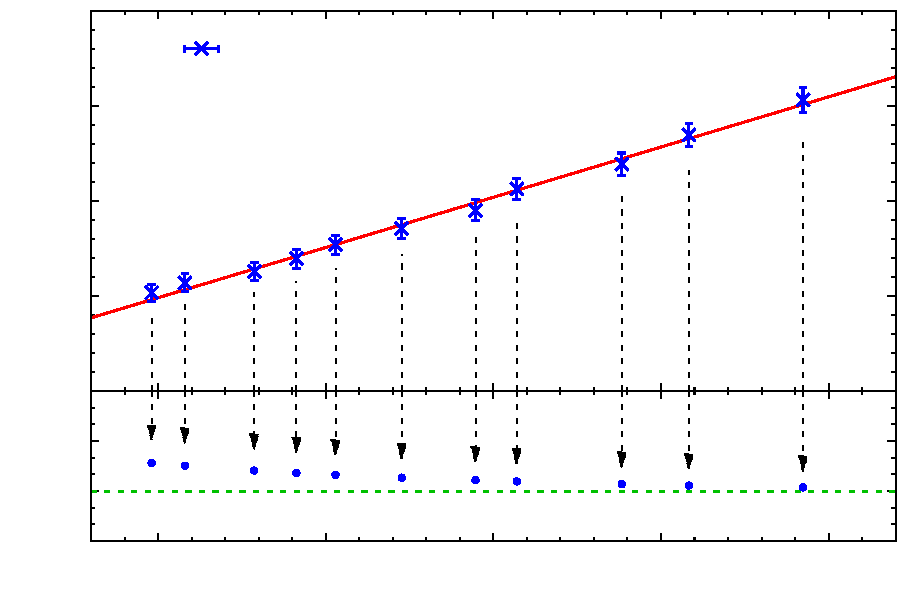
\includegraphics{pics/gad_10cm}}%
    \gplfronttext
  \end{picture}%
\endgroup
}
	\caption{Gadolinium absorption lines.}
	\label{fig:gad_10cm}
\end{figure}

\begin{figure}
	\centering
	\resizebox{0.6\linewidth}{!}{% GNUPLOT: LaTeX picture with Postscript
\begingroup
  \makeatletter
  \providecommand\color[2][]{%
    \GenericError{(gnuplot) \space\space\space\@spaces}{%
      Package color not loaded in conjunction with
      terminal option `colourtext'%
    }{See the gnuplot documentation for explanation.%
    }{Either use 'blacktext' in gnuplot or load the package
      color.sty in LaTeX.}%
    \renewcommand\color[2][]{}%
  }%
  \providecommand\includegraphics[2][]{%
    \GenericError{(gnuplot) \space\space\space\@spaces}{%
      Package graphicx or graphics not loaded%
    }{See the gnuplot documentation for explanation.%
    }{The gnuplot epslatex terminal needs graphicx.sty or graphics.sty.}%
    \renewcommand\includegraphics[2][]{}%
  }%
  \providecommand\rotatebox[2]{#2}%
  \@ifundefined{ifGPcolor}{%
    \newif\ifGPcolor
    \GPcolortrue
  }{}%
  \@ifundefined{ifGPblacktext}{%
    \newif\ifGPblacktext
    \GPblacktexttrue
  }{}%
  % define a \g@addto@macro without @ in the name:
  \let\gplgaddtomacro\g@addto@macro
  % define empty templates for all commands taking text:
  \gdef\gplbacktext{}%
  \gdef\gplfronttext{}%
  \makeatother
  \ifGPblacktext
    % no textcolor at all
    \def\colorrgb#1{}%
    \def\colorgray#1{}%
  \else
    % gray or color?
    \ifGPcolor
      \def\colorrgb#1{\color[rgb]{#1}}%
      \def\colorgray#1{\color[gray]{#1}}%
      \expandafter\def\csname LTw\endcsname{\color{white}}%
      \expandafter\def\csname LTb\endcsname{\color{black}}%
      \expandafter\def\csname LTa\endcsname{\color{black}}%
      \expandafter\def\csname LT0\endcsname{\color[rgb]{1,0,0}}%
      \expandafter\def\csname LT1\endcsname{\color[rgb]{0,1,0}}%
      \expandafter\def\csname LT2\endcsname{\color[rgb]{0,0,1}}%
      \expandafter\def\csname LT3\endcsname{\color[rgb]{1,0,1}}%
      \expandafter\def\csname LT4\endcsname{\color[rgb]{0,1,1}}%
      \expandafter\def\csname LT5\endcsname{\color[rgb]{1,1,0}}%
      \expandafter\def\csname LT6\endcsname{\color[rgb]{0,0,0}}%
      \expandafter\def\csname LT7\endcsname{\color[rgb]{1,0.3,0}}%
      \expandafter\def\csname LT8\endcsname{\color[rgb]{0.5,0.5,0.5}}%
    \else
      % gray
      \def\colorrgb#1{\color{black}}%
      \def\colorgray#1{\color[gray]{#1}}%
      \expandafter\def\csname LTw\endcsname{\color{white}}%
      \expandafter\def\csname LTb\endcsname{\color{black}}%
      \expandafter\def\csname LTa\endcsname{\color{black}}%
      \expandafter\def\csname LT0\endcsname{\color{black}}%
      \expandafter\def\csname LT1\endcsname{\color{black}}%
      \expandafter\def\csname LT2\endcsname{\color{black}}%
      \expandafter\def\csname LT3\endcsname{\color{black}}%
      \expandafter\def\csname LT4\endcsname{\color{black}}%
      \expandafter\def\csname LT5\endcsname{\color{black}}%
      \expandafter\def\csname LT6\endcsname{\color{black}}%
      \expandafter\def\csname LT7\endcsname{\color{black}}%
      \expandafter\def\csname LT8\endcsname{\color{black}}%
    \fi
  \fi
    \setlength{\unitlength}{0.0500bp}%
    \ifx\gptboxheight\undefined%
      \newlength{\gptboxheight}%
      \newlength{\gptboxwidth}%
      \newsavebox{\gptboxtext}%
    \fi%
    \setlength{\fboxrule}{0.5pt}%
    \setlength{\fboxsep}{1pt}%
\begin{picture}(7200.00,5040.00)%
    \gplgaddtomacro\gplbacktext{%
      \csname LTb\endcsname%%
      \put(849,595){\makebox(0,0)[r]{\strut{}$0$}}%
      \csname LTb\endcsname%%
      \put(849,1465){\makebox(0,0)[r]{\strut{}$5000$}}%
      \csname LTb\endcsname%%
      \put(849,2335){\makebox(0,0)[r]{\strut{}$10000$}}%
      \csname LTb\endcsname%%
      \put(849,3206){\makebox(0,0)[r]{\strut{}$15000$}}%
      \csname LTb\endcsname%%
      \put(849,4076){\makebox(0,0)[r]{\strut{}$20000$}}%
      \csname LTb\endcsname%%
      \put(849,4946){\makebox(0,0)[r]{\strut{}$25000$}}%
      \csname LTb\endcsname%%
      \put(951,409){\makebox(0,0){\strut{}$260$}}%
      \csname LTb\endcsname%%
      \put(1607,409){\makebox(0,0){\strut{}$265$}}%
      \csname LTb\endcsname%%
      \put(2263,409){\makebox(0,0){\strut{}$270$}}%
      \csname LTb\endcsname%%
      \put(2918,409){\makebox(0,0){\strut{}$275$}}%
      \csname LTb\endcsname%%
      \put(3574,409){\makebox(0,0){\strut{}$280$}}%
      \csname LTb\endcsname%%
      \put(4230,409){\makebox(0,0){\strut{}$285$}}%
      \csname LTb\endcsname%%
      \put(4886,409){\makebox(0,0){\strut{}$290$}}%
      \csname LTb\endcsname%%
      \put(5541,409){\makebox(0,0){\strut{}$295$}}%
      \csname LTb\endcsname%%
      \put(6197,409){\makebox(0,0){\strut{}$300$}}%
      \csname LTb\endcsname%%
      \put(6299,595){\makebox(0,0)[l]{\strut{}$0$}}%
      \csname LTb\endcsname%%
      \put(6299,1030){\makebox(0,0)[l]{\strut{}$0.1$}}%
      \csname LTb\endcsname%%
      \put(6299,1465){\makebox(0,0)[l]{\strut{}$0.2$}}%
      \csname LTb\endcsname%%
      \put(6299,1900){\makebox(0,0)[l]{\strut{}$0.3$}}%
      \csname LTb\endcsname%%
      \put(6299,2335){\makebox(0,0)[l]{\strut{}$0.4$}}%
      \csname LTb\endcsname%%
      \put(6299,2771){\makebox(0,0)[l]{\strut{}$0.5$}}%
      \csname LTb\endcsname%%
      \put(6299,3206){\makebox(0,0)[l]{\strut{}$0.6$}}%
      \csname LTb\endcsname%%
      \put(6299,3641){\makebox(0,0)[l]{\strut{}$0.7$}}%
      \csname LTb\endcsname%%
      \put(6299,4076){\makebox(0,0)[l]{\strut{}$0.8$}}%
      \csname LTb\endcsname%%
      \put(6299,4511){\makebox(0,0)[l]{\strut{}$0.9$}}%
      \csname LTb\endcsname%%
      \put(6299,4946){\makebox(0,0)[l]{\strut{}$1$}}%
    }%
    \gplgaddtomacro\gplfronttext{%
      \csname LTb\endcsname%%
      \put(153,2770){\rotatebox{-270}{\makebox(0,0){\strut{}Intensity}}}%
      \csname LTb\endcsname%%
      \put(6911,2770){\rotatebox{-270}{\makebox(0,0){\strut{}Absorbance}}}%
      \csname LTb\endcsname%%
      \put(3574,130){\makebox(0,0){\strut{}Wavelength (nm)}}%
      \csname LTb\endcsname%%
      \put(5613,4779){\makebox(0,0)[r]{\strut{}Pure water}}%
      \csname LTb\endcsname%%
      \put(5613,4593){\makebox(0,0)[r]{\strut{}Gd water}}%
      \csname LTb\endcsname%%
      \put(5613,4407){\makebox(0,0)[r]{\strut{}Absorbance}}%
    }%
    \gplbacktext
    \put(0,0){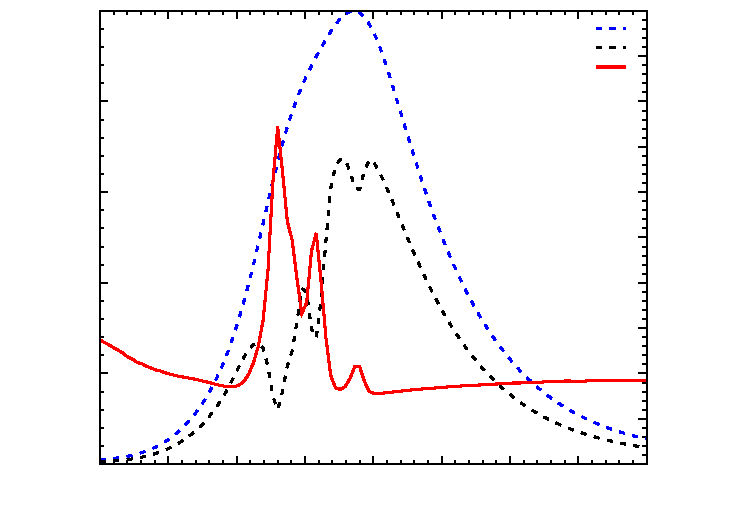
\includegraphics{pics/abs_example}}%
    \gplfronttext
  \end{picture}%
\endgroup
}
	\caption{Gadolinium absorption lines.}
	\label{fig:gad_10cm}
\end{figure}


The first concept of tracking gadolinium concentration in water using absorbance spectrum %
was tested using a 1\,cm cell in a commercial spectrophotometer Shimadzu UV2600, %
in which an initial sample of 0.2\,\% Gd water is diluited to obtain different concentration levels.
The gadolinium loaded sample is compared to a pure water one to compute the absorbance spectrum.
The result is...? And linear fit.
The Shimadzu spectrophotometer uses a grating system to select very narrow windows of electromagnetic spectrum %
both at the source and at the detection, which is done by a photomultiplier.
The source at UV wavelengths is provided by a deuterium lamp, integrated in the spectrometer.
The advantage of this technique is that very high resolution can be achieved, %
but a scan wavelength per wavelength is done, taking one measurement at the time.
This process can be quite slow and the gain from the resolution is not so relevant.
We tested different model of other commercial spectrometers, without integrated source and %
with a grating system such that the input light is spread out on a linear CCD.
Doing so, the whole spectrum to which the spectroemter is sensitive to, is taken simultaneously.
The measurement is then only limited to the reading speed rate of the spectrometer.
A set of consecutive measurement can be taken and averaging them the error can also be estimated.
After testing different models from different companies, we purchased an Ocean HDX spectrometer.
The advantage of this spectrometer is a very high light throughput thanks to a toroidal mirroring system %
which reduces stray light and maximises the input light.
In addition to this, the sensor has a high dynamic range, which is the determing factor %
on the absorbance measurement.
Wavelength resolution is not as important, because we use the relative position of the gadolinium peaks %
to determine the absorbance.

\begin{figure}
	\centering
	\resizebox{\linewidth}{!}{% GNUPLOT: LaTeX picture with Postscript
\begingroup
  \makeatletter
  \providecommand\color[2][]{%
    \GenericError{(gnuplot) \space\space\space\@spaces}{%
      Package color not loaded in conjunction with
      terminal option `colourtext'%
    }{See the gnuplot documentation for explanation.%
    }{Either use 'blacktext' in gnuplot or load the package
      color.sty in LaTeX.}%
    \renewcommand\color[2][]{}%
  }%
  \providecommand\includegraphics[2][]{%
    \GenericError{(gnuplot) \space\space\space\@spaces}{%
      Package graphicx or graphics not loaded%
    }{See the gnuplot documentation for explanation.%
    }{The gnuplot epslatex terminal needs graphicx.sty or graphics.sty.}%
    \renewcommand\includegraphics[2][]{}%
  }%
  \providecommand\rotatebox[2]{#2}%
  \@ifundefined{ifGPcolor}{%
    \newif\ifGPcolor
    \GPcolortrue
  }{}%
  \@ifundefined{ifGPblacktext}{%
    \newif\ifGPblacktext
    \GPblacktexttrue
  }{}%
  % define a \g@addto@macro without @ in the name:
  \let\gplgaddtomacro\g@addto@macro
  % define empty templates for all commands taking text:
  \gdef\gplbacktext{}%
  \gdef\gplfronttext{}%
  \makeatother
  \ifGPblacktext
    % no textcolor at all
    \def\colorrgb#1{}%
    \def\colorgray#1{}%
  \else
    % gray or color?
    \ifGPcolor
      \def\colorrgb#1{\color[rgb]{#1}}%
      \def\colorgray#1{\color[gray]{#1}}%
      \expandafter\def\csname LTw\endcsname{\color{white}}%
      \expandafter\def\csname LTb\endcsname{\color{black}}%
      \expandafter\def\csname LTa\endcsname{\color{black}}%
      \expandafter\def\csname LT0\endcsname{\color[rgb]{1,0,0}}%
      \expandafter\def\csname LT1\endcsname{\color[rgb]{0,1,0}}%
      \expandafter\def\csname LT2\endcsname{\color[rgb]{0,0,1}}%
      \expandafter\def\csname LT3\endcsname{\color[rgb]{1,0,1}}%
      \expandafter\def\csname LT4\endcsname{\color[rgb]{0,1,1}}%
      \expandafter\def\csname LT5\endcsname{\color[rgb]{1,1,0}}%
      \expandafter\def\csname LT6\endcsname{\color[rgb]{0,0,0}}%
      \expandafter\def\csname LT7\endcsname{\color[rgb]{1,0.3,0}}%
      \expandafter\def\csname LT8\endcsname{\color[rgb]{0.5,0.5,0.5}}%
    \else
      % gray
      \def\colorrgb#1{\color{black}}%
      \def\colorgray#1{\color[gray]{#1}}%
      \expandafter\def\csname LTw\endcsname{\color{white}}%
      \expandafter\def\csname LTb\endcsname{\color{black}}%
      \expandafter\def\csname LTa\endcsname{\color{black}}%
      \expandafter\def\csname LT0\endcsname{\color{black}}%
      \expandafter\def\csname LT1\endcsname{\color{black}}%
      \expandafter\def\csname LT2\endcsname{\color{black}}%
      \expandafter\def\csname LT3\endcsname{\color{black}}%
      \expandafter\def\csname LT4\endcsname{\color{black}}%
      \expandafter\def\csname LT5\endcsname{\color{black}}%
      \expandafter\def\csname LT6\endcsname{\color{black}}%
      \expandafter\def\csname LT7\endcsname{\color{black}}%
      \expandafter\def\csname LT8\endcsname{\color{black}}%
    \fi
  \fi
    \setlength{\unitlength}{0.0500bp}%
    \ifx\gptboxheight\undefined%
      \newlength{\gptboxheight}%
      \newlength{\gptboxwidth}%
      \newsavebox{\gptboxtext}%
    \fi%
    \setlength{\fboxrule}{0.5pt}%
    \setlength{\fboxsep}{1pt}%
\begin{picture}(14400.00,5760.00)%
    \gplgaddtomacro\gplbacktext{%
      \csname LTb\endcsname%%
      \put(618,624){\makebox(0,0)[r]{\strut{}0}}%
      \csname LTb\endcsname%%
      \put(618,1296){\makebox(0,0)[r]{\strut{}0.2}}%
      \csname LTb\endcsname%%
      \put(618,1969){\makebox(0,0)[r]{\strut{}0.4}}%
      \csname LTb\endcsname%%
      \put(618,2641){\makebox(0,0)[r]{\strut{}0.6}}%
      \csname LTb\endcsname%%
      \put(618,3313){\makebox(0,0)[r]{\strut{}0.8}}%
      \csname LTb\endcsname%%
      \put(618,3985){\makebox(0,0)[r]{\strut{}1}}%
      \csname LTb\endcsname%%
      \put(618,4658){\makebox(0,0)[r]{\strut{}1.2}}%
      \csname LTb\endcsname%%
      \put(618,5330){\makebox(0,0)[r]{\strut{}1.4}}%
      \csname LTb\endcsname%%
      \put(720,102){\makebox(0,0){\strut{}$240$}}%
      \csname LTb\endcsname%%
      \put(1697,102){\makebox(0,0){\strut{}$250$}}%
      \csname LTb\endcsname%%
      \put(2674,102){\makebox(0,0){\strut{}$260$}}%
      \csname LTb\endcsname%%
      \put(3651,102){\makebox(0,0){\strut{}$270$}}%
      \csname LTb\endcsname%%
      \put(4628,102){\makebox(0,0){\strut{}$280$}}%
      \csname LTb\endcsname%%
      \put(5605,102){\makebox(0,0){\strut{}$290$}}%
      \csname LTb\endcsname%%
      \put(6582,102){\makebox(0,0){\strut{}$300$}}%
    }%
    \gplgaddtomacro\gplfronttext{%
      \csname LTb\endcsname%%
      \put(126,2977){\rotatebox{-270}{\makebox(0,0){\strut{}Absorbance}}}%
      \csname LTb\endcsname%%
      \put(6975,3453){\makebox(0,0)[r]{\strut{}0.016\%}}%
      \csname LTb\endcsname%%
      \put(6975,3639){\makebox(0,0)[r]{\strut{}0.018\%}}%
      \csname LTb\endcsname%%
      \put(6975,3825){\makebox(0,0)[r]{\strut{}0.020\%}}%
      \csname LTb\endcsname%%
      \put(6975,4011){\makebox(0,0)[r]{\strut{}0.022\%}}%
      \csname LTb\endcsname%%
      \put(6975,4197){\makebox(0,0)[r]{\strut{}0.024\%}}%
      \csname LTb\endcsname%%
      \put(6975,4383){\makebox(0,0)[r]{\strut{}0.030\%}}%
      \csname LTb\endcsname%%
      \put(6975,4569){\makebox(0,0)[r]{\strut{}0.050\%}}%
      \csname LTb\endcsname%%
      \put(6975,4755){\makebox(0,0)[r]{\strut{}0.100\%}}%
      \csname LTb\endcsname%%
      \put(6975,4941){\makebox(0,0)[r]{\strut{}0.160\%}}%
      \csname LTb\endcsname%%
      \put(6975,5127){\makebox(0,0)[r]{\strut{}0.180\%}}%
      \csname LTb\endcsname%%
      \put(6975,5313){\makebox(0,0)[r]{\strut{}0.200\%}}%
      \csname LTb\endcsname%%
      \put(6975,5499){\makebox(0,0)[r]{\strut{}0.220\%}}%
    }%
    \gplgaddtomacro\gplbacktext{%
      \csname LTb\endcsname%%
      \put(7457,624){\makebox(0,0)[r]{\strut{}}}%
      \csname LTb\endcsname%%
      \put(7457,1296){\makebox(0,0)[r]{\strut{}}}%
      \csname LTb\endcsname%%
      \put(7457,1969){\makebox(0,0)[r]{\strut{}}}%
      \csname LTb\endcsname%%
      \put(7457,2641){\makebox(0,0)[r]{\strut{}}}%
      \csname LTb\endcsname%%
      \put(7457,3313){\makebox(0,0)[r]{\strut{}}}%
      \csname LTb\endcsname%%
      \put(7457,3985){\makebox(0,0)[r]{\strut{}}}%
      \csname LTb\endcsname%%
      \put(7457,4658){\makebox(0,0)[r]{\strut{}}}%
      \csname LTb\endcsname%%
      \put(7457,5330){\makebox(0,0)[r]{\strut{}}}%
      \csname LTb\endcsname%%
      \put(7559,102){\makebox(0,0){\strut{}$240$}}%
      \csname LTb\endcsname%%
      \put(8529,102){\makebox(0,0){\strut{}$250$}}%
      \csname LTb\endcsname%%
      \put(9499,102){\makebox(0,0){\strut{}$260$}}%
      \csname LTb\endcsname%%
      \put(10469,102){\makebox(0,0){\strut{}$270$}}%
      \csname LTb\endcsname%%
      \put(11438,102){\makebox(0,0){\strut{}$280$}}%
      \csname LTb\endcsname%%
      \put(12408,102){\makebox(0,0){\strut{}$290$}}%
      \csname LTb\endcsname%%
      \put(13378,102){\makebox(0,0){\strut{}$300$}}%
      \csname LTb\endcsname%%
      \put(14348,102){\makebox(0,0){\strut{}$310$}}%
      \csname LTb\endcsname%%
      \put(10954,4658){\makebox(0,0){\strut{}\shortstack{background \\ subtraction}}}%
    }%
    \gplgaddtomacro\gplfronttext{%
      \csname LTb\endcsname%%
      \put(7457,2977){\rotatebox{-270}{\makebox(0,0){\strut{}}}}%
    }%
    \gplbacktext
    \put(0,0){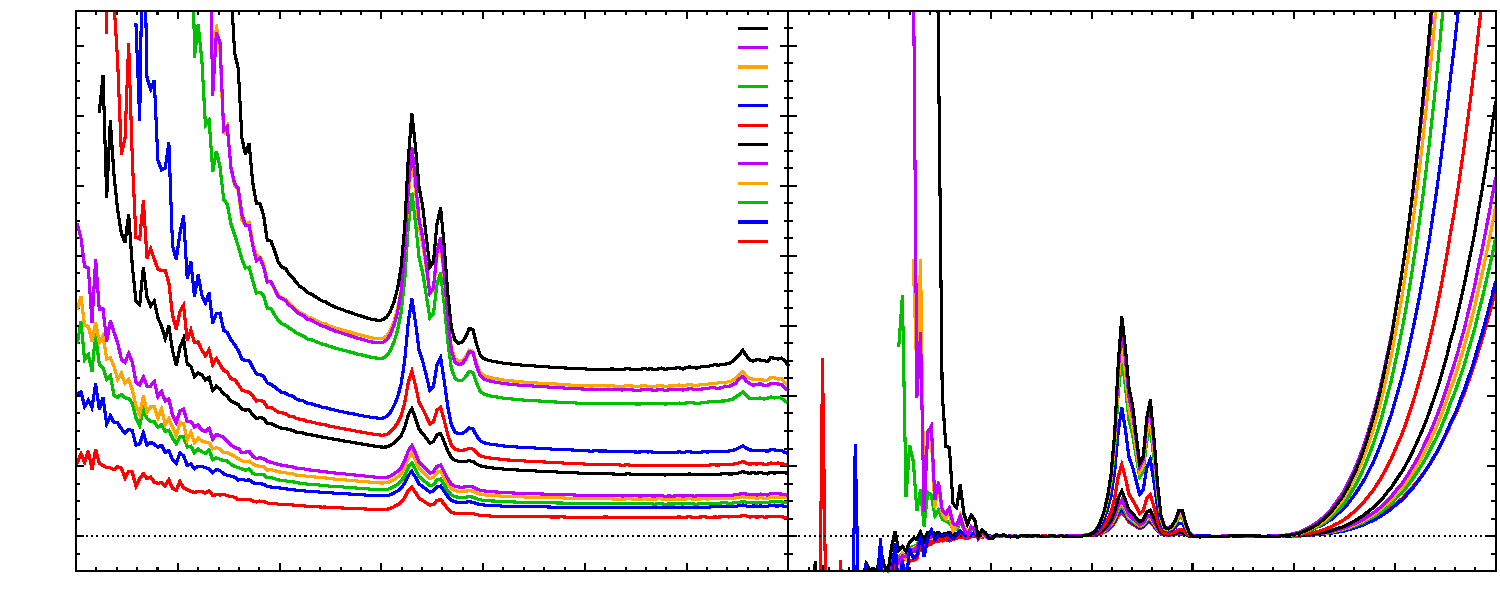
\includegraphics{pics/polyfit}}%
    \gplfronttext
  \end{picture}%
\endgroup
}
	\caption{Gadolinium absorption lines.}
	\label{fig:gad_fit}
\end{figure}

The first prototype based on a 10 cm cell for 0.2$\%$ Gadolinium sulphate doping achieved %
a $3\%$ concentration measurement resolution ($1\%$ neutron capture efficiency) %
at the target concentration in comparison to the $3.5\%$ currently achieved via a manual mass spectrometer method.

This device was intended for deployment in EGADS in Japan but the Gadolinium sulphate %
concentration was changed to $0.02\%$ in preparation for Super-K phase 1 loading.
Therefore work progressed to building the version 2 prototype of GAD for %
sensitivity to $0.02\%$, by increasing the volume to $\approx 1$ meter.

This prototype has been successfully built and tested and shown a concentration measurement %
resolution of $1\%$ at both $0.02\%$ and $0.2\%$ doping.


